\documentclass[11pt]{article}

% --- Page layout ---
\usepackage[a4paper,margin=2cm]{geometry}

% --- Typography and section formatting ---
\usepackage{titlesec}
\titleformat{\section}{\normalfont\Large\bfseries}{}{0pt}{}
\titleformat{\subsection}{\normalfont\large\bfseries}{}{0pt}{}
\usepackage{parskip}

% --- Figures and tables ---
\usepackage{graphicx}
\usepackage{float}
\usepackage{booktabs}
\usepackage{caption}
\usepackage{subcaption}
\captionsetup[figure]{justification=centering}
\usepackage{url}
\usepackage{subcaption}
\usepackage[table]{xcolor}

% --- Citations ---
\usepackage{endnotes}
\let\footnote=\endnote
\usepackage{bibentry}
\nobibliography*

% --- Document starts here ---
\begin{document}
	
	\begin{center}
		\LARGE\textbf{Ship Detection Pipeline for Smart Port Monitoring}
	\end{center}
	
	\section*{Introduction}
	
	Maritime trade remains a cornerstone of global commerce, with over 80\% of goods transported by sea\endnote{\bibentry{unctad2023}}. Efficient port operations are essential for supply chain stability, and real-time vessel monitoring is a key feature of emerging smart port systems. Satellite-based ship detection complements Automatic Identification System (AIS) data by identifying vessels that do not broadcast their location, thereby supporting traffic management, berth allocation, and maritime security.
	
	Recent advances in deep learning have markedly improved ship detection in optical satellite imagery, shifting from traditional sliding-window classifiers to convolutional neural networks (CNNs) and object detection frameworks\endnote{\bibentry{patel2022}}. Kanjir et al. (2018) provided a comprehensive review showing that CNN-based models consistently outperform classical image processing techniques in maritime surveillance. Zhang et al. (2019) demonstrated the effectiveness of fine-tuning a Faster R-CNN architecture, originally pre-trained on ImageNet, for ship detection in high-resolution imagery. Their model outperformed both YOLOv2 and traditional approaches, particularly in identifying small or clustered vessels. Building on this, Bakırcı (2025) applied the latest YOLOv9 model to maritime scenes, achieving high accuracy and real-time performance under challenging conditions such as wakes and dense traffic. While one-stage detectors like YOLO offer speed advantages, detecting small, densely packed vessels remains a persistent challenge. Zhao et al. (2024) reviewed methods to address this issue, including multi-scale feature extraction and attention mechanisms. Similarly, Shi et al. (2025) introduced Ship-YOLO, a modified YOLO architecture tailored for maritime imagery, which achieved improved performance in complex environments.
	
	Together, these studies highlight the growing maturity of deep learning approaches for ship detection and their potential for smart port application. However, challenges remain in adapting pre-trained models to limited training data and ensuring robust performance across diverse imagery conditions. This study investigates whether pre-trained CNNs can be fine-tuned to accurately detect ships in satellite imagery of port environments. Using the ShipsNet dataset, we evaluate the performance of fine-tuned VGG11, ResNet50, and EfficientNet-B0 models for binary ship classification, and extend detection to full-scene satellite images through a sliding-window inference pipeline.
	
	\section*{Data and Methods}
	
	\subsection*{2.1 Dataset}
	
	This study uses the ShipsNet dataset, a publicly available collection of labelled satellite imagery derived from PlanetScope scenes over San Francisco Bay and San Pedro Bay\endnote{\bibentry{shipsnet2025}}. It comprises 4,000 RGB image chips, each measuring 80 × 80 pixels, with a ground sampling distance of approximately 3 meters. Each chip is annotated as either \textit{ship} (1) or \textit{no-ship} (0).
	
	The \textit{ship} class contains 1,000 images centred on the main body of a vessel, spanning a range of sizes, orientations, and atmospheric conditions. The 3,000 \textit{no-ship} images include an equal mix of random land cover, partial ship instances, and visually ambiguous features—such as bright pixels or strong linear structures—known to mislead classifiers. The dataset also includes eight full-scene satellite images of port environments, which simulate real-world deployment and enable spatially explicit validation via sliding-window detection across continuous imagery.
	
	\subsection*{2.2 Data Preparation}
	
	We performed a stratified split of the dataset into 80\% training and 20\% test sets, preserving the original class distribution. The training set was then balanced by randomly upsampling the minority \textit{ship} class to match the number of \textit{no-ship} samples, while the test set retained its natural imbalance to support unbiased model evaluation.
	
	To enhance generalisability and simulate common variations in optical satellite imagery, we applied data augmentation to the training set. Each chip had a 50\% probability of undergoing horizontal or vertical flips, random rotation within $\pm20^\circ$, and colour jittering to adjust brightness, contrast, and saturation. Augmented images were resized to 224 × 224 pixels to match the input dimensions of pre-trained CNNs and were normalised using the mean and standard deviation of the ImageNet dataset.
	
	\subsection*{2.3 Model Training and Evaluation}
	
	We adopted a transfer learning approach to leverage the feature extraction capabilities of pre-trained models, a standard practice when working with limited training data\endnote{\bibentry{patel2022}}. Three CNN architectures—VGG11, ResNet50, and EfficientNet-B0—were fine-tuned for binary classification by replacing their final fully connected layers with two-class output heads corresponding to the \textit{ship} and \textit{no-ship} labels. To mitigate overfitting, the convolutional base layers were frozen during training, and only the classifier head was updated. This feature extraction strategy supports efficient learning from small, augmented datasets.
	
	All models were trained for 30 epochs using the Adam optimiser with a learning rate of $5 \times 10^{-4}$ and a batch size of 24. Accuracy and binary cross-entropy loss were tracked on both training and test sets after each epoch. Early stopping with a patience of five epochs was applied to halt training when test loss no longer improved, reducing unnecessary computation. Training and validation curves were plotted to monitor convergence. Random seeds were fixed across training routines to ensure reproducibility.
	
	Model performance was evaluated on the held-out test set using standard metrics: accuracy, precision, recall, and F1 score. Confusion matrices were also generated to provide a detailed breakdown of classification outcomes.
		
	\subsection*{2.4 Ship Detection in Full-Scene Imagery}
	
	Beyond chip-level classification, we implemented a sliding-window approach to detect ships in larger satellite scenes. A fixed 80 × 80 pixel window was moved across each full-scene image at a predefined stride of 20 pixels. Each window was classified by the trained model, and those with a predicted probability greater than 0.95 for the \textit{ship} class were retained as detections.
	
	To address overlapping detections around individual ships, Non-Maximum Suppression (NMS) was applied post hoc using an Intersection-over-Union (IoU) threshold of 0.1. NMS retains the highest-confidence prediction and discards nearby detections that overlap beyond the specified IoU, which measures the ratio of the intersecting area to the union of two bounding boxes. This conservative threshold was chosen to reflect the small object size relative to the image and to minimise false suppression of adjacent true positives.
	
	\subsection*{2.5 Model Interpretability}
	
	To validate model behaviour, we applied occlusion-based attribution using the \texttt{Captum} library. A 20 × 20 pixel sliding mask was passed over individual test images, systematically occluding regions to measure changes in prediction confidence. This yielded sensitivity maps that highlighted the areas most influential in the classification decision. Additionally, we generated probability heatmaps across full-scene satellite images, visualising predicted ship likelihoods over broader port environments. Together, these techniques offered a multi-scale view of model focus, aligning with best practices in explainable AI and confirming that predictions were based on relevant image features rather than background artefacts.
	
	\begin{figure}[H]
		\centering
		\caption{Label Distribution}
		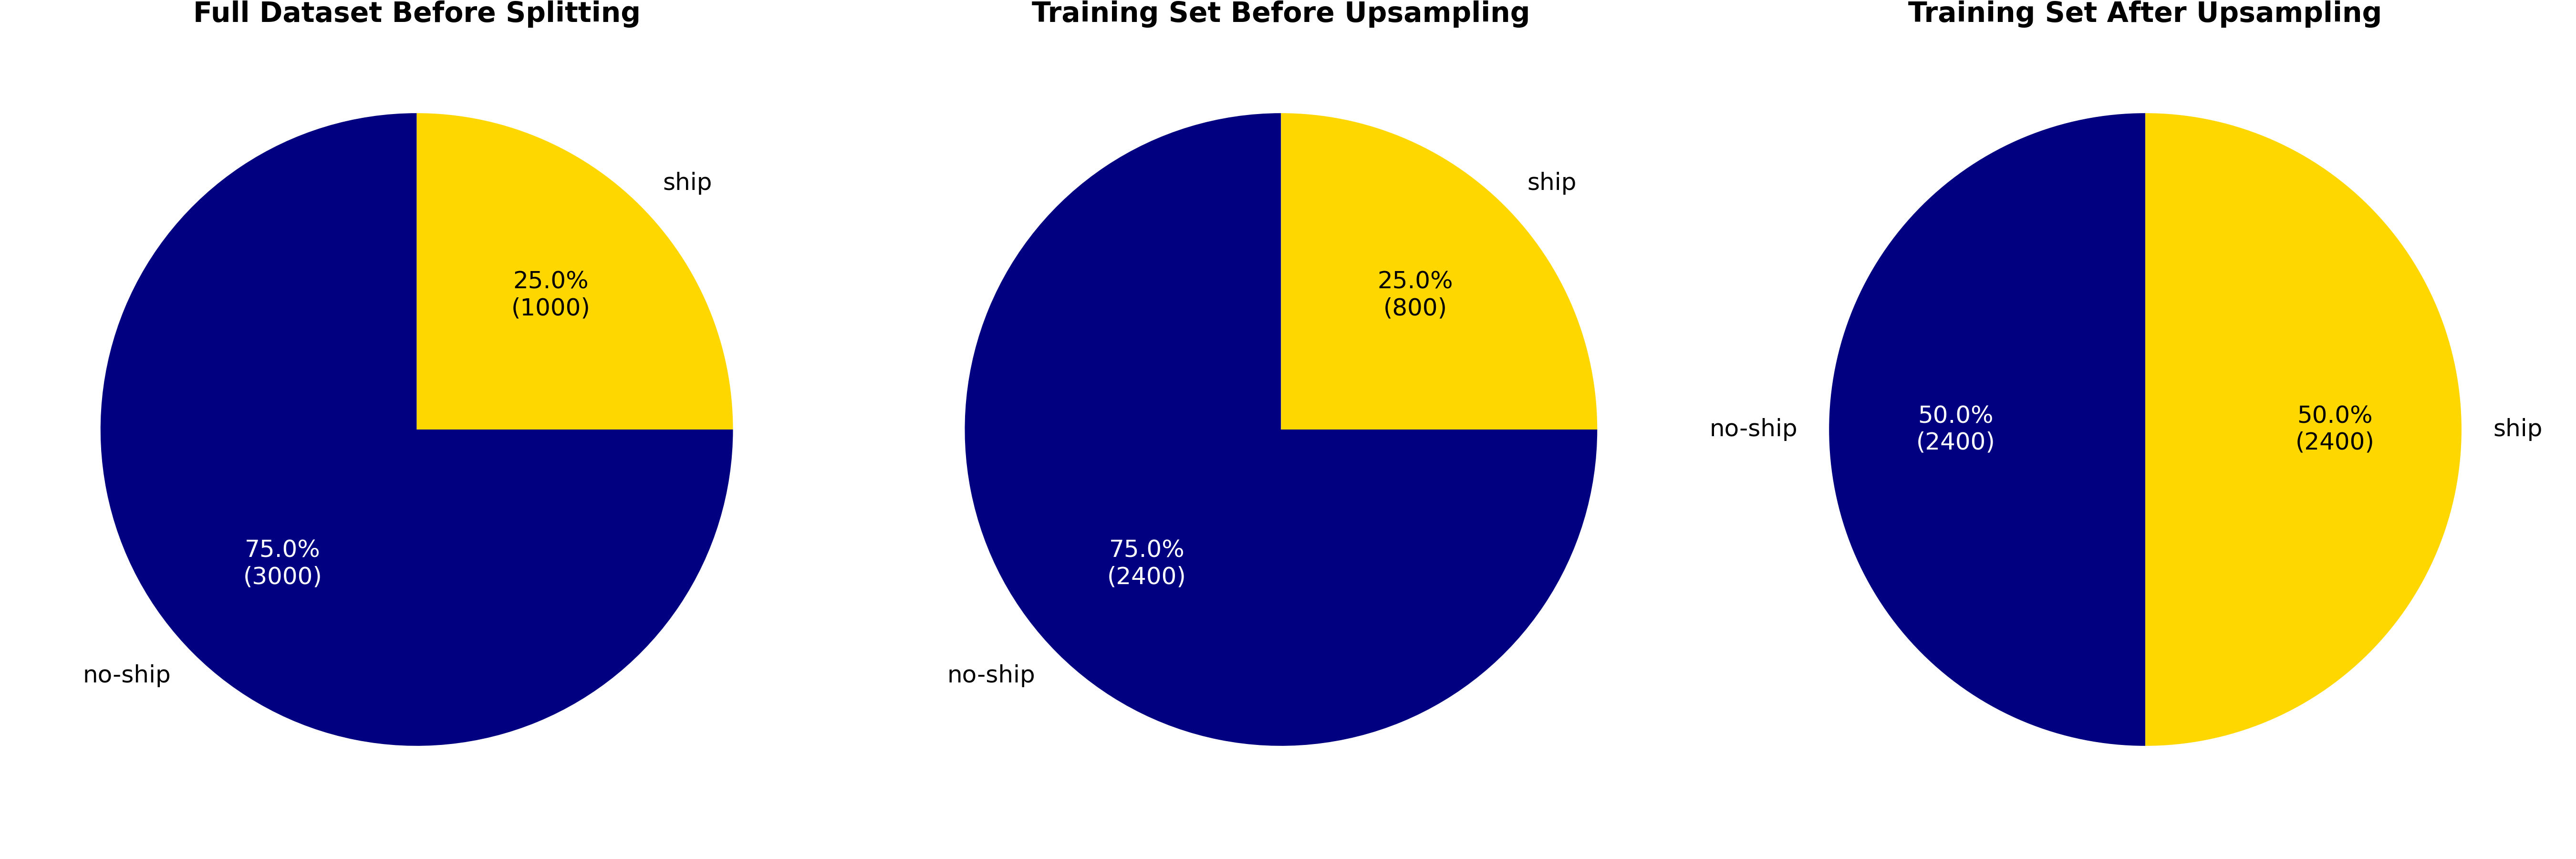
\includegraphics[width=\linewidth]{assets/label_distribution/label_distribution.png}
	\end{figure}
	
	\begin{figure}[H]
		\centering
		\caption{\textit{ship} and \textit{no-ship} Samples}
		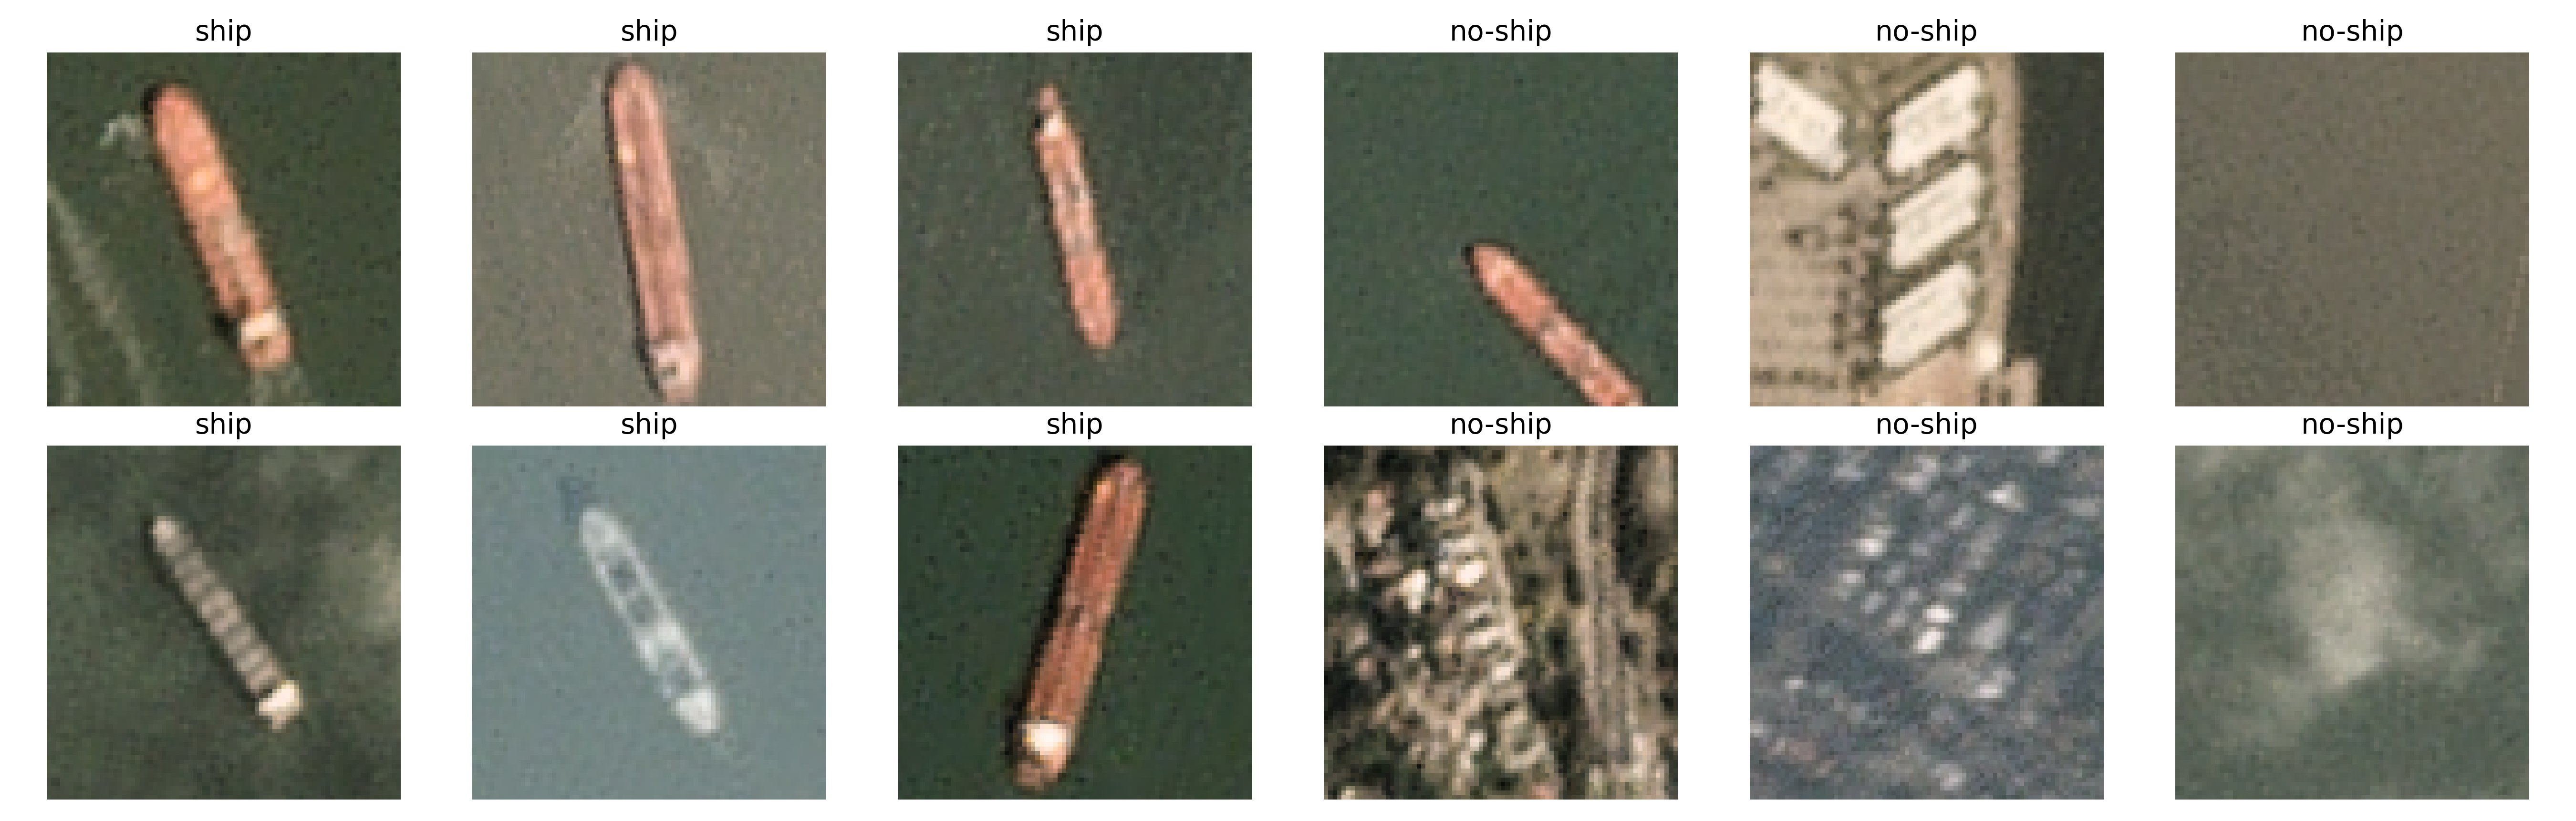
\includegraphics[width=\linewidth]{assets/data_example/ship_vs_noship_examples.png}
	\end{figure}
	
	\begin{figure}[H]
		\centering
		\caption{Data Augmentation}
		\includegraphics[width=\linewidth]{assets/data_augmentation/data_augmentation_comparison.png}
	\end{figure}
	
	\section*{Results and Discussion}
	
	\begin{figure}[H]
		\centering
		\caption{Evaluation Results}
		
		% Table of performance metrics
		\begin{subfigure}[b]{0.95\textwidth}
			\centering
			\makebox[\textwidth]{
			\renewcommand{\arraystretch}{1.5}
			\small
			\begin{tabular}{lccccccc}
				\specialrule{1.2pt}{0pt}{0pt}
				\textbf{Model} & \textbf{Accuracy} & \textbf{Precision} & \textbf{Recall} & \textbf{F1 Score} & \textbf{Best Epoch} & \textbf{Train Loss} & \textbf{Test Loss} \\
				\midrule
				VGG11            & 0.9500 & 0.9200 & 0.9400 & 0.9300 & 24/30 & 0.2147 & 0.1361 \\
				\midrule
				ResNet50         & 0.9200 & 0.8800 & 0.9200 & 0.9000 & 11/30 & 0.1981 & 0.1900 \\
				\midrule
				EfficientNet-B0  & 0.8800 & 0.8300 & 0.9000 & 0.8500 & 13/30 & 0.2357 & 0.2644 \\
				\specialrule{1.2pt}{0pt}{0pt}
			\end{tabular}
			}
			\vspace{0.75em}
			\caption{Performance Metrics and Losses at Best Epoch}
		\end{subfigure}
		
		\vspace{1em}
		
		\setcounter{subfigure}{1}
		
		% Confusion Matrices
		\begin{subfigure}[b]{\textwidth}
			\centering
			\begin{subfigure}[b]{0.32\textwidth}
				\centering
				\captionsetup{labelformat=empty}
				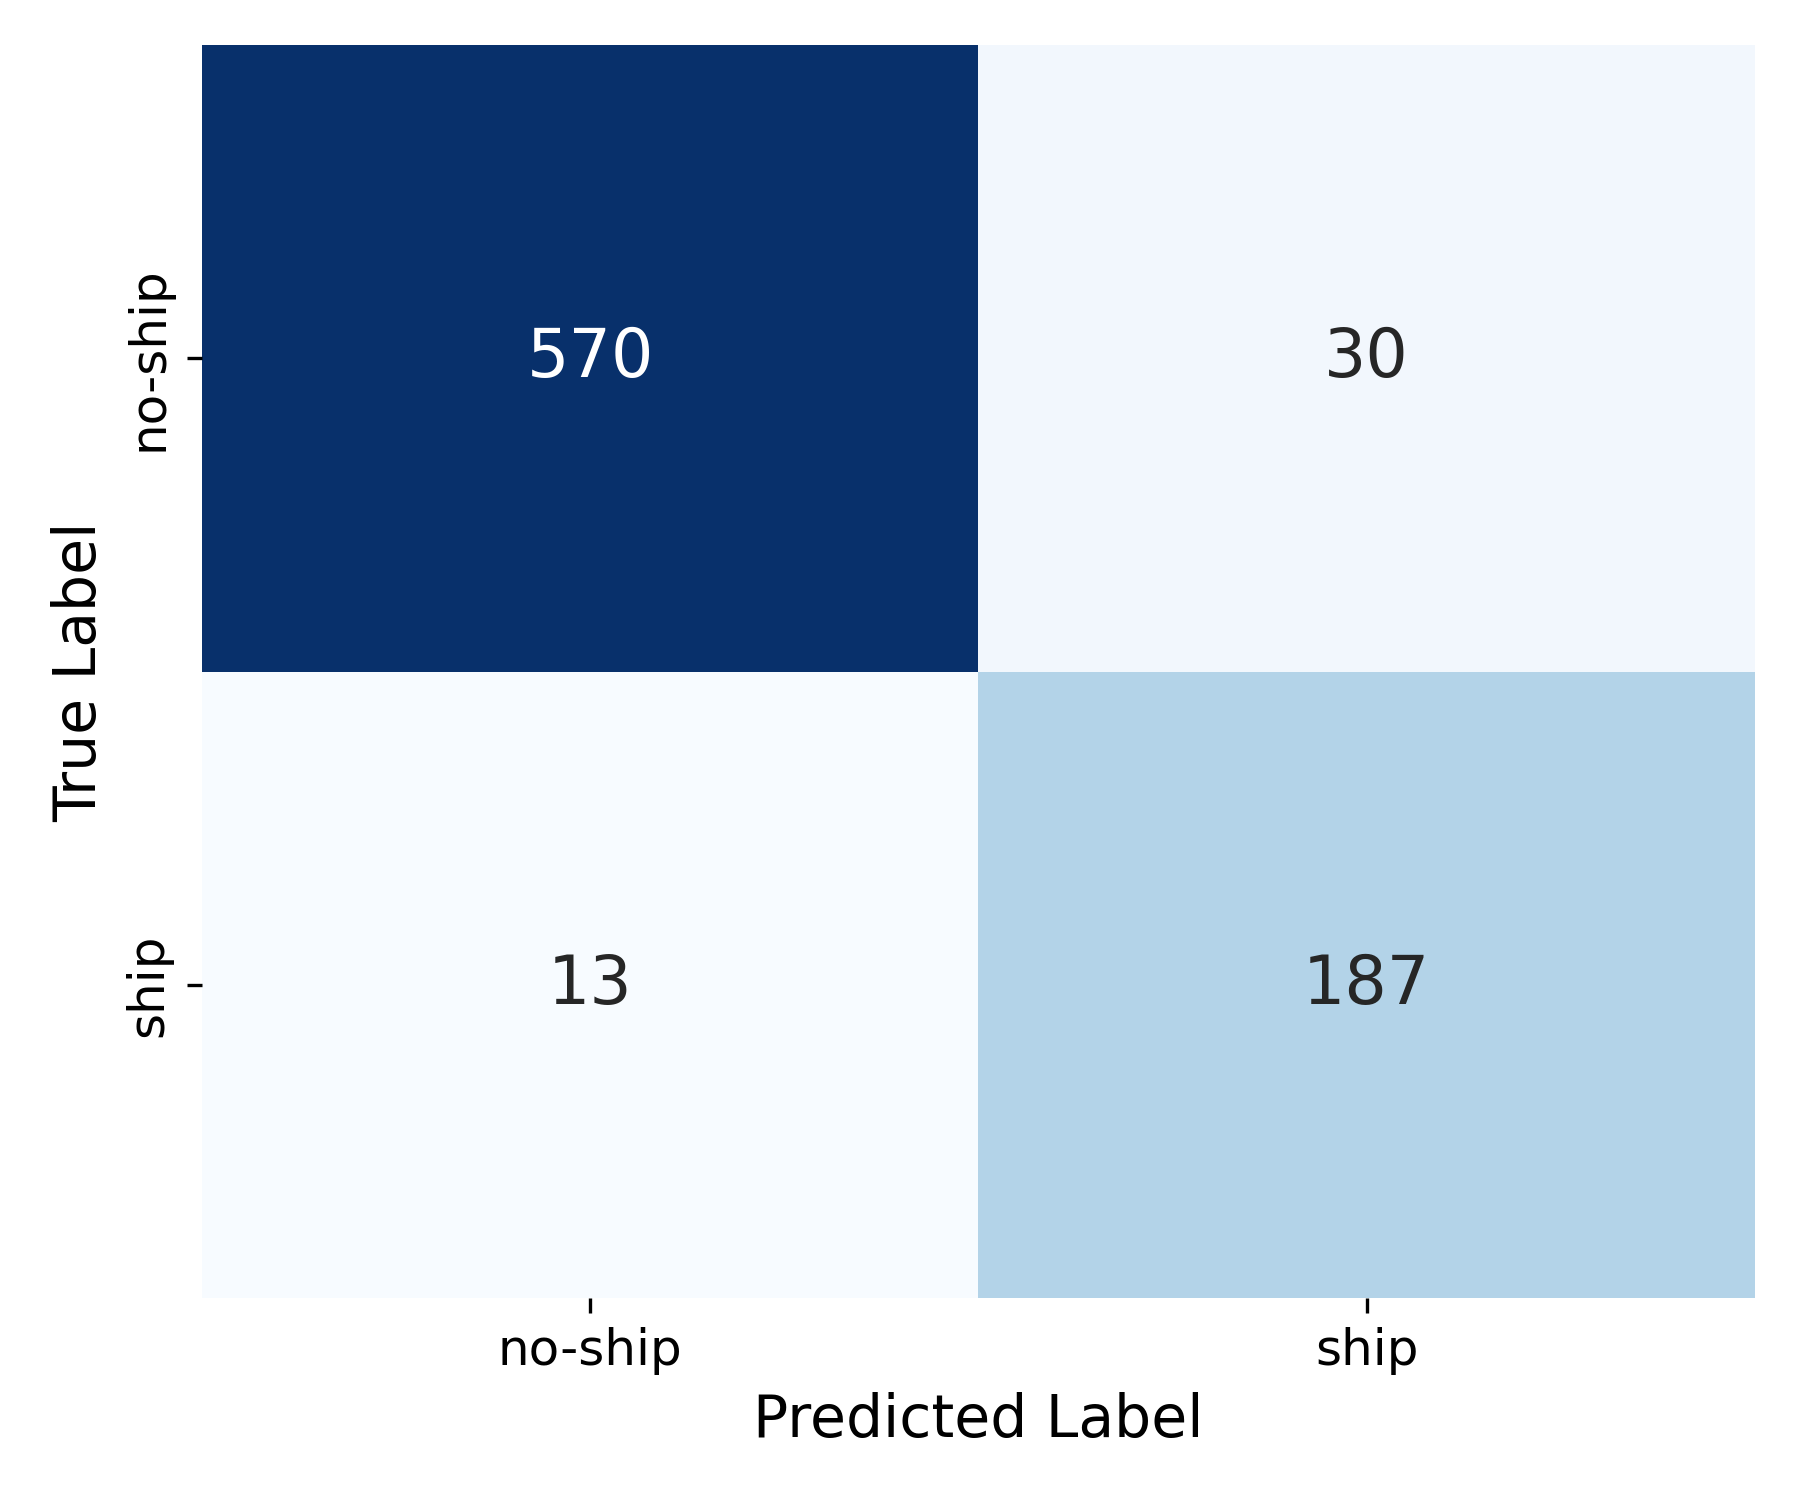
\includegraphics[width=\textwidth]{assets/confusion_matrix/vgg11_confusion_matrix.png}
				\caption*{1. VGG11}
			\end{subfigure}
			\hfill
			\begin{subfigure}[b]{0.32\textwidth}
				\centering
				\captionsetup{labelformat=empty}
				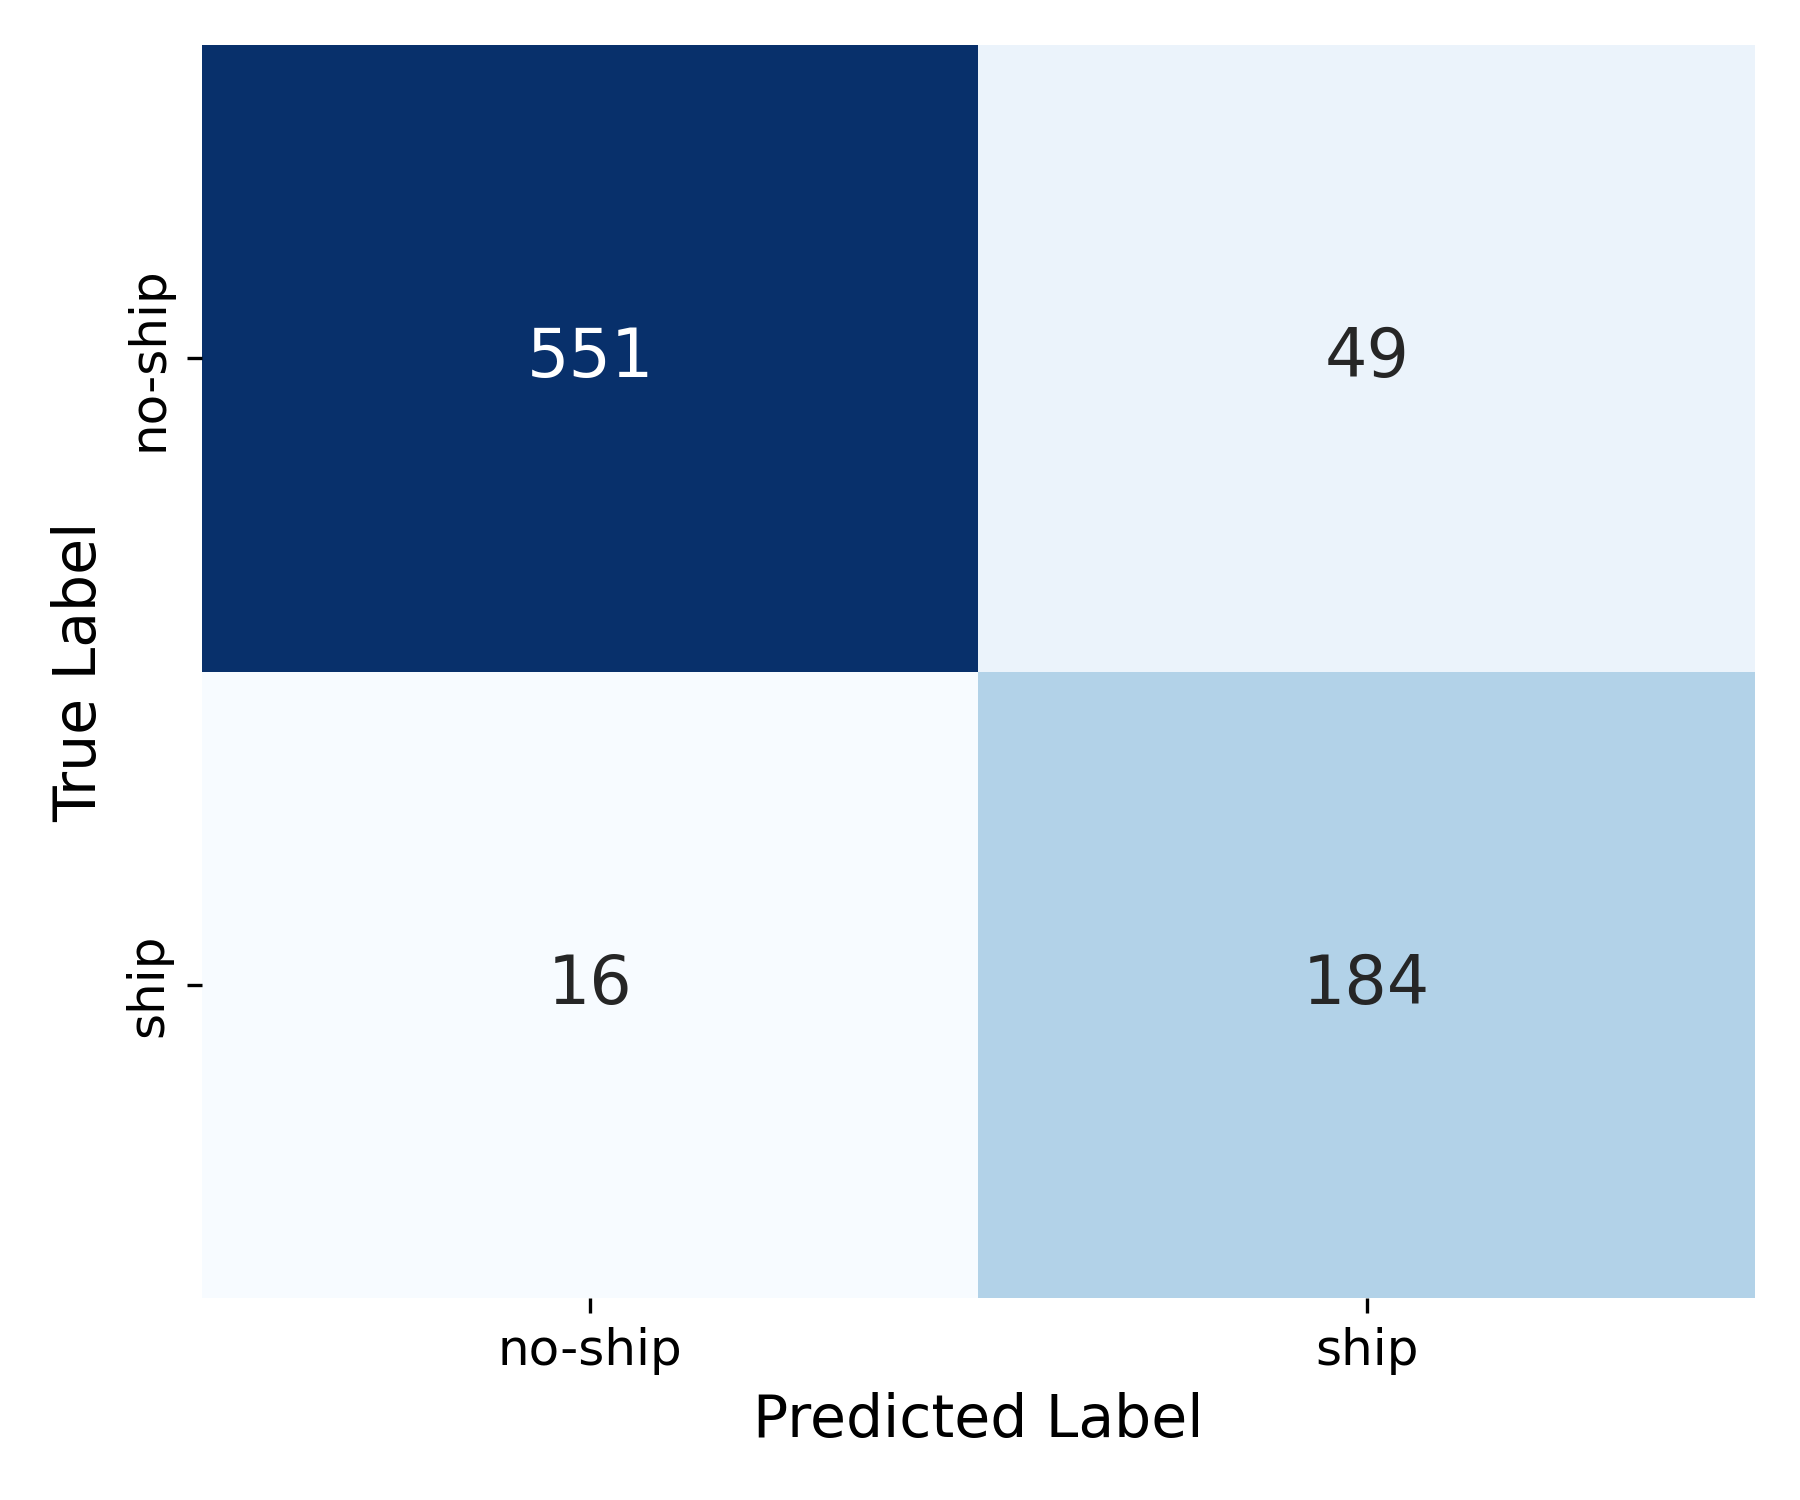
\includegraphics[width=\textwidth]{assets/confusion_matrix/resnet50_confusion_matrix.png}
				\caption*{2. ResNet50}
			\end{subfigure}
			\hfill
			\begin{subfigure}[b]{0.32\textwidth}
				\centering
				\captionsetup{labelformat=empty}
				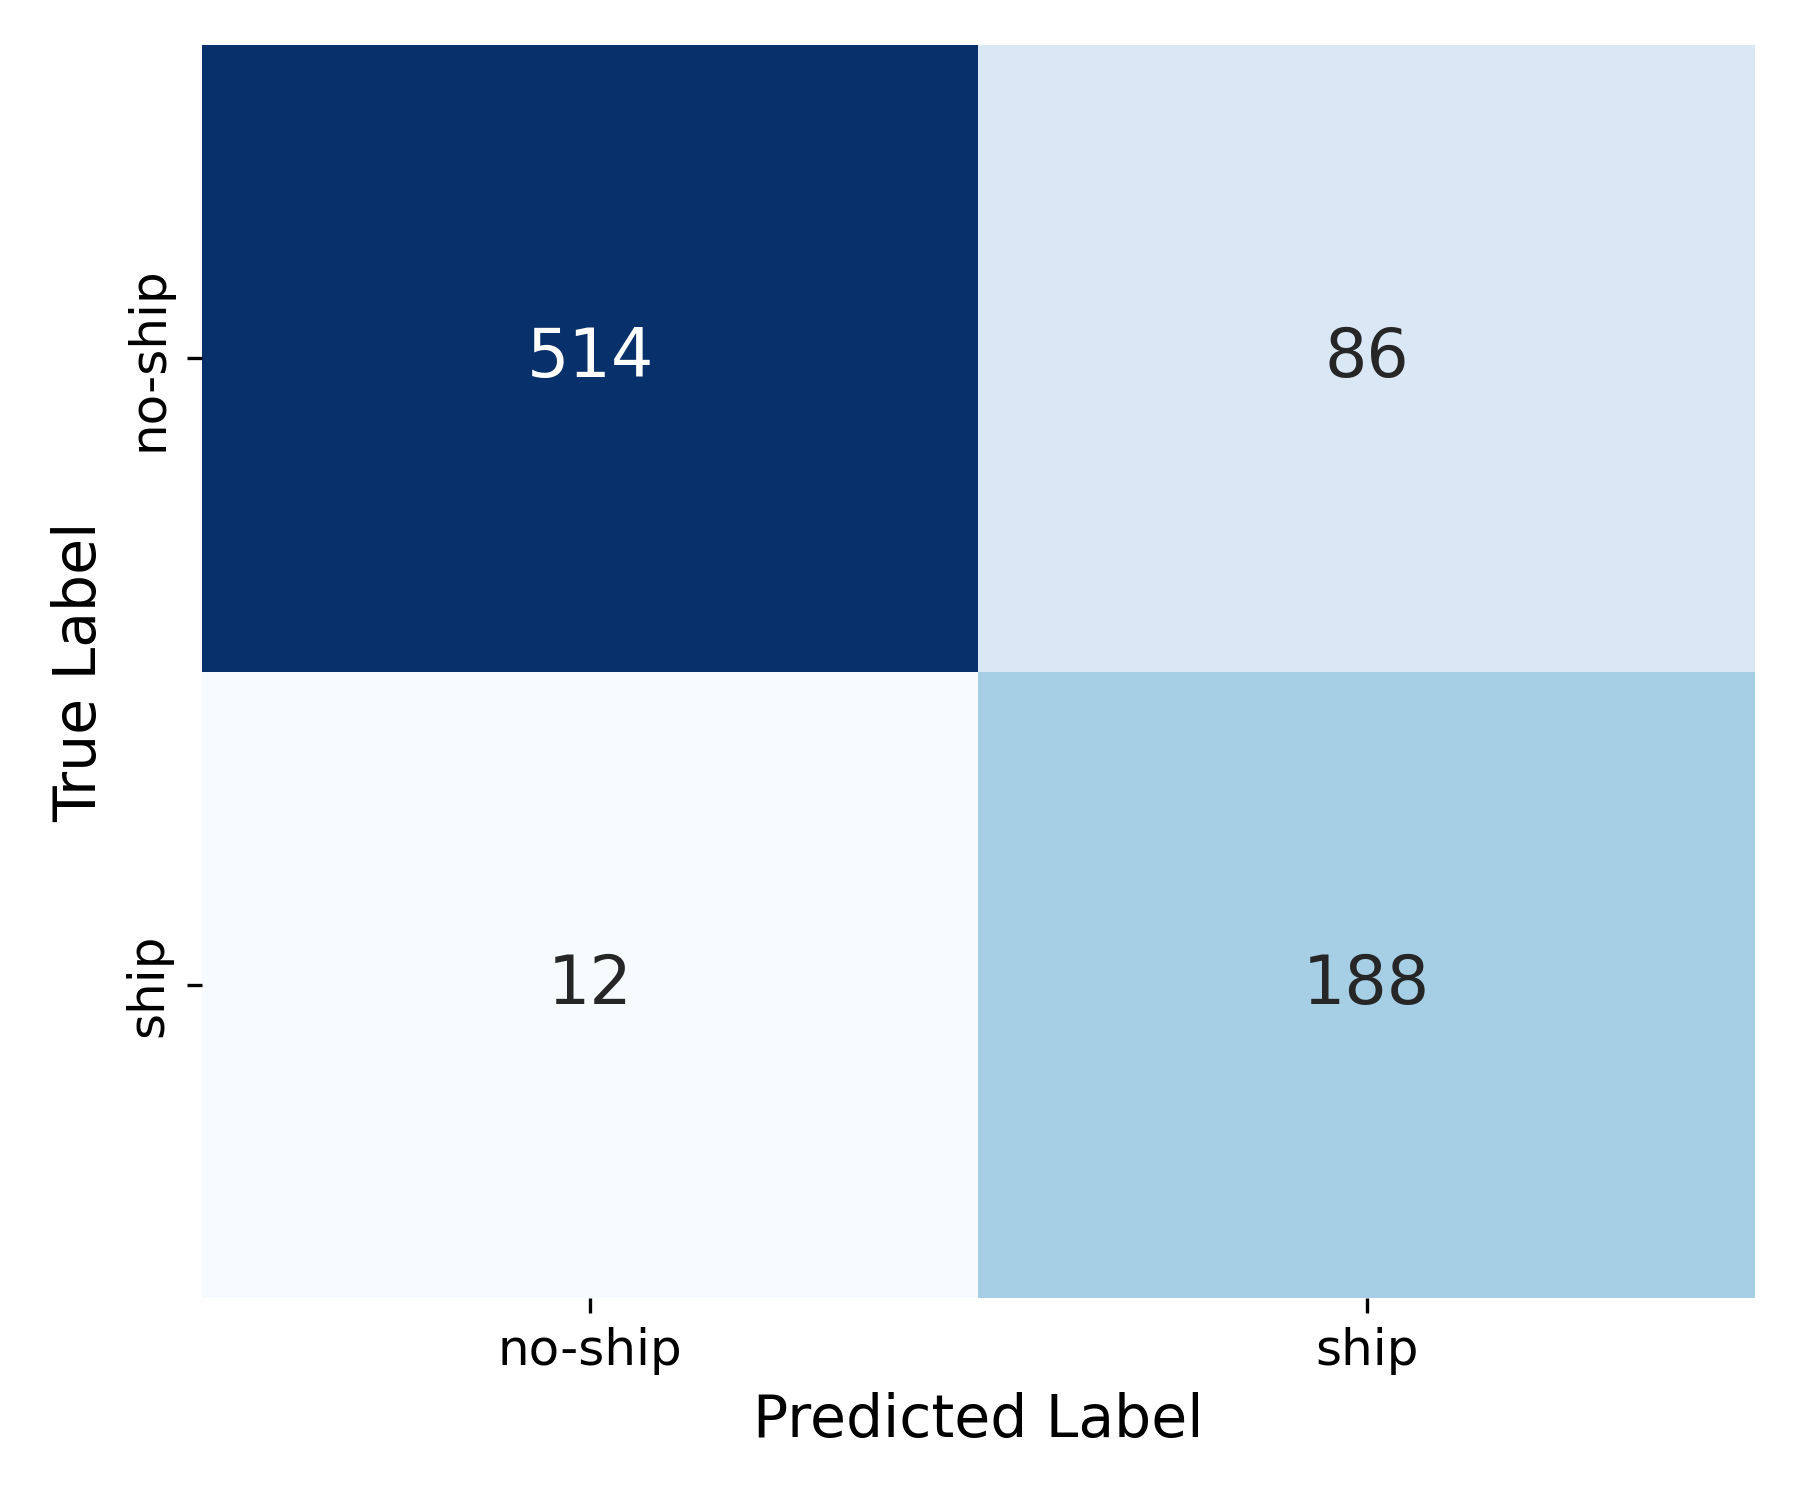
\includegraphics[width=\textwidth]{assets/confusion_matrix/efficientnet_confusion_matrix.png}
				\caption*{3. EfficientNet-B0}
			\end{subfigure}
			\caption{Confusion Matrices}
		\end{subfigure}
		
	\end{figure}
	
	\begin{figure}[H]
		\centering
		\caption{Training and Validation Accuracy and Loss Curves}
		
		\vspace{-1em}
		
		% VGG11
		\begin{subfigure}[b]{0.49\textwidth}
			\centering
			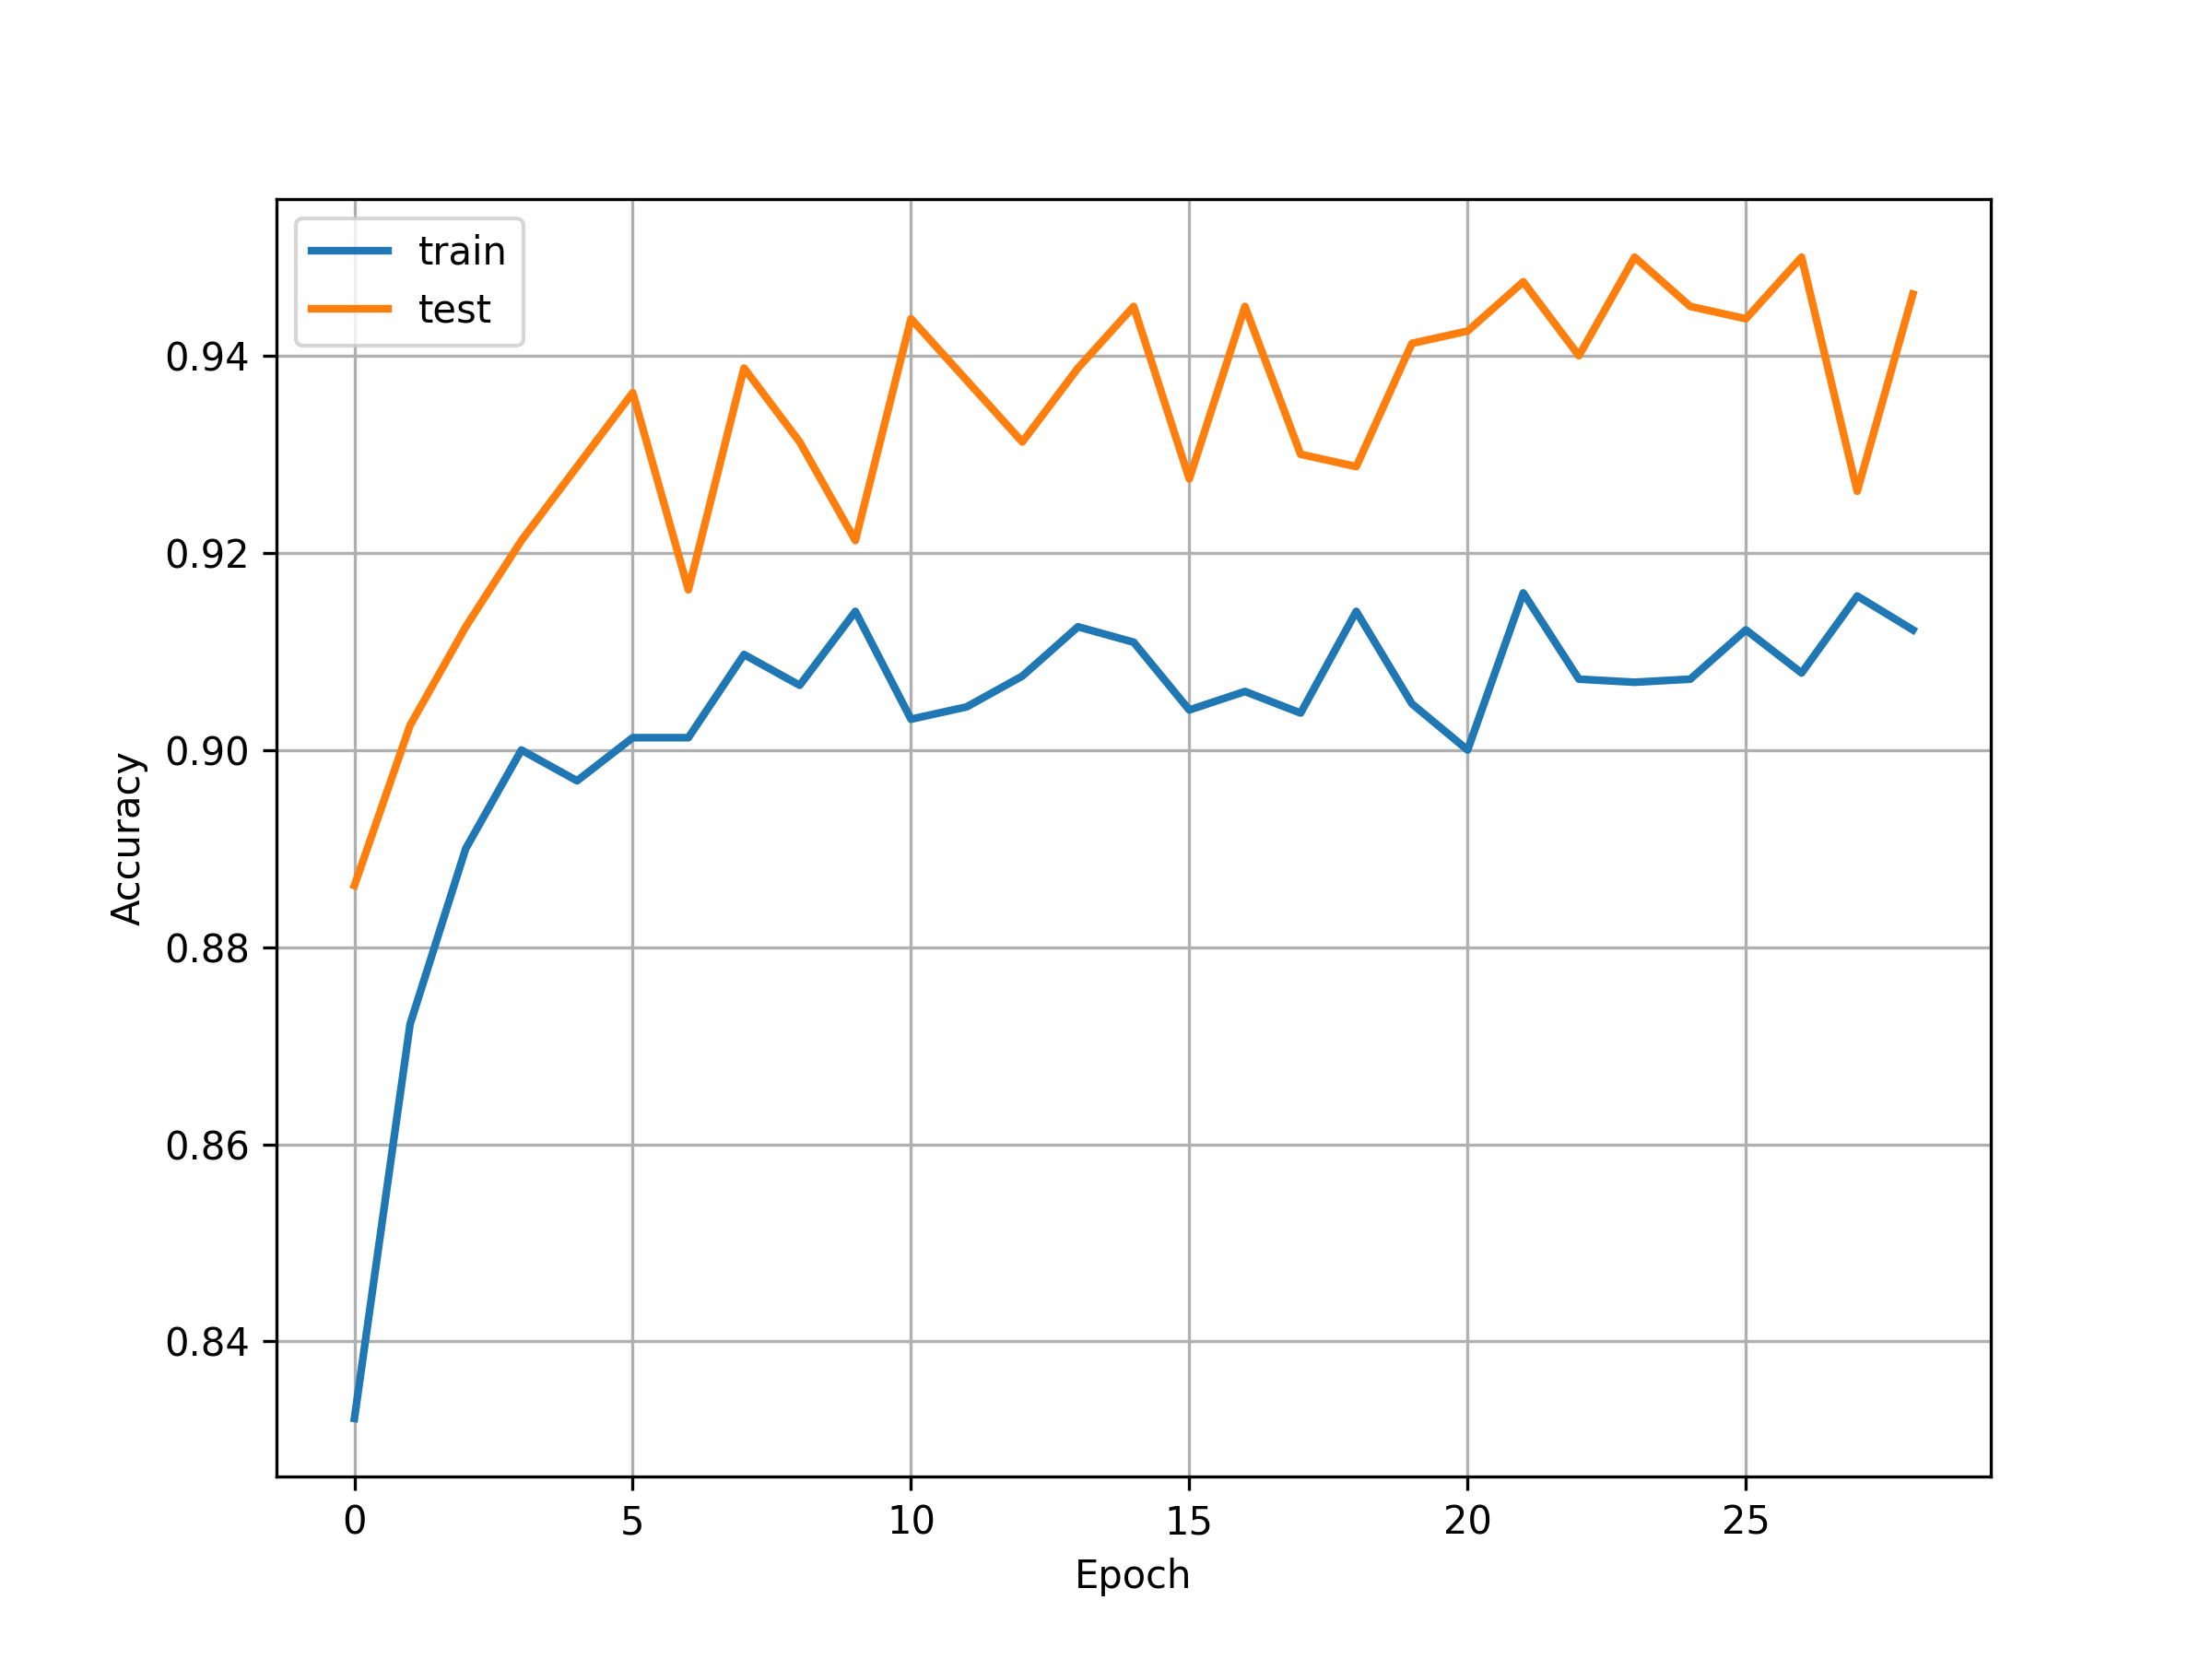
\includegraphics[width=\linewidth, trim=20 10 20 10, clip]{assets/accuracy_curve/vgg11_accuracy_curve.png}
			\caption{VGG11 - Accuracy}
		\end{subfigure}
		\hfill
		\begin{subfigure}[b]{0.49\textwidth}
			\centering
			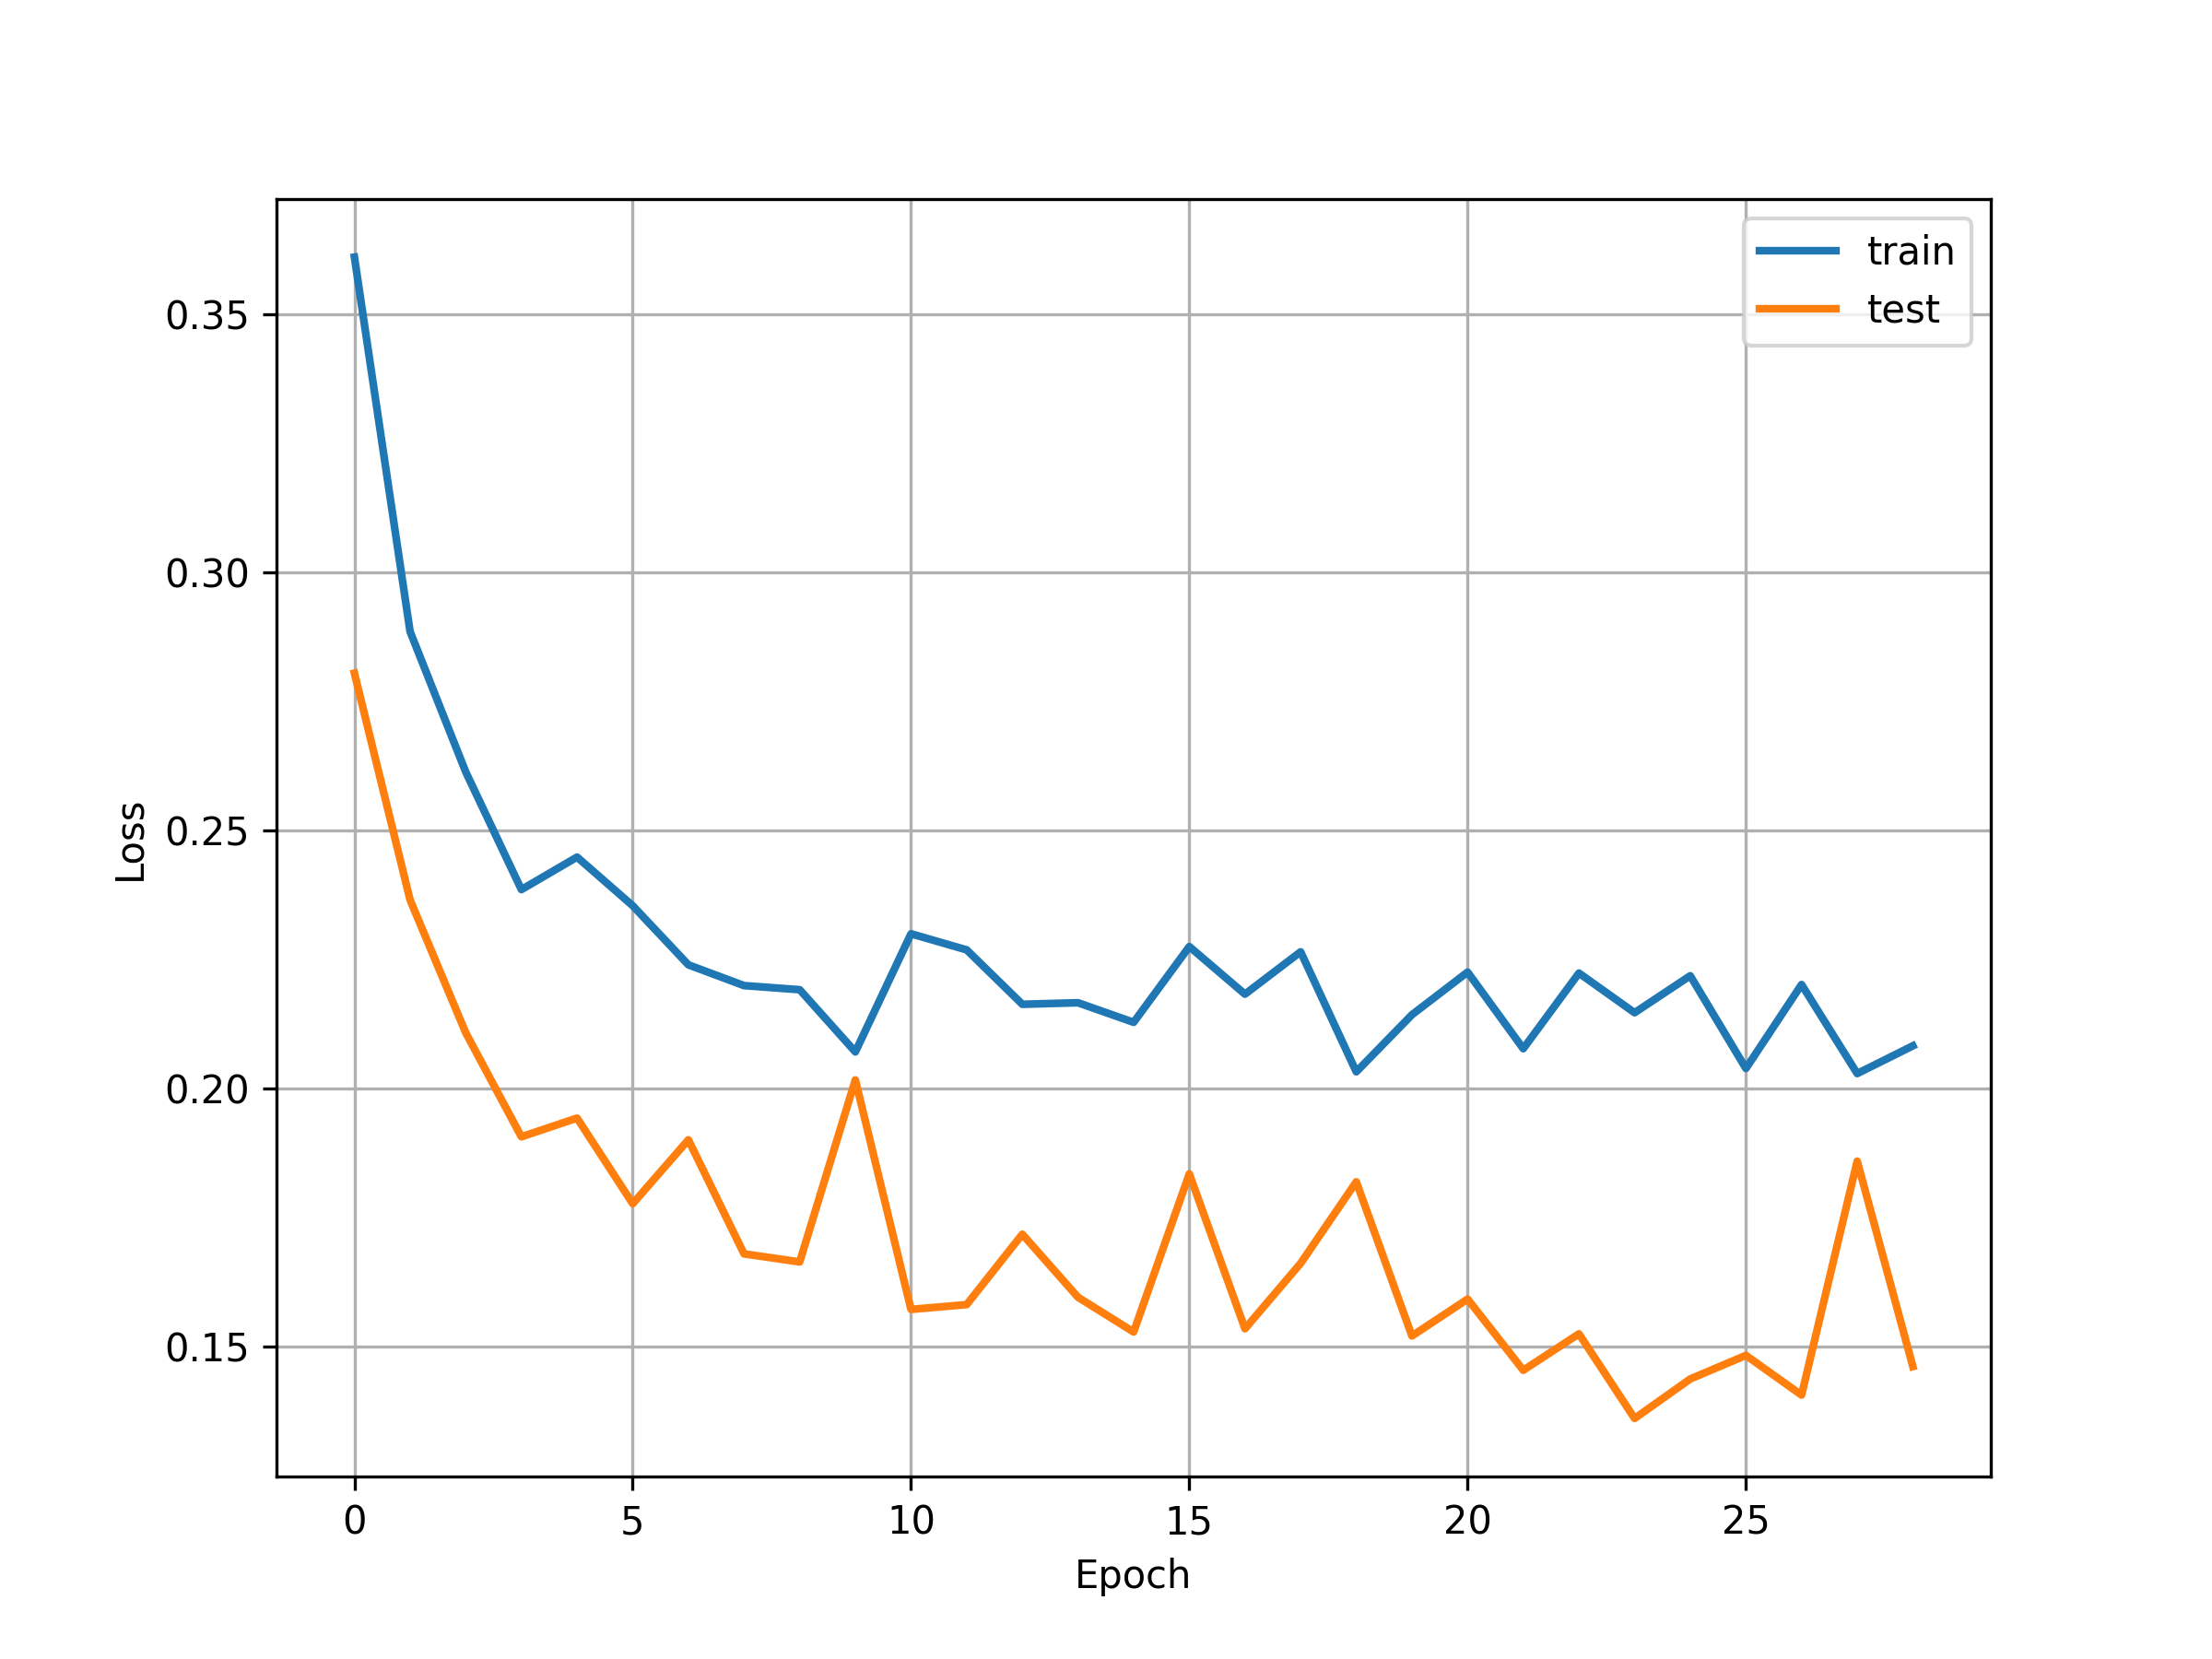
\includegraphics[width=\linewidth, trim=20 10 20 10, clip]{assets/loss_curve/vgg11_loss_curve.png}
			\caption{VGG11 - Loss}
		\end{subfigure}
		
		
		% ResNet50
		\begin{subfigure}[b]{0.49\textwidth}
			\centering
			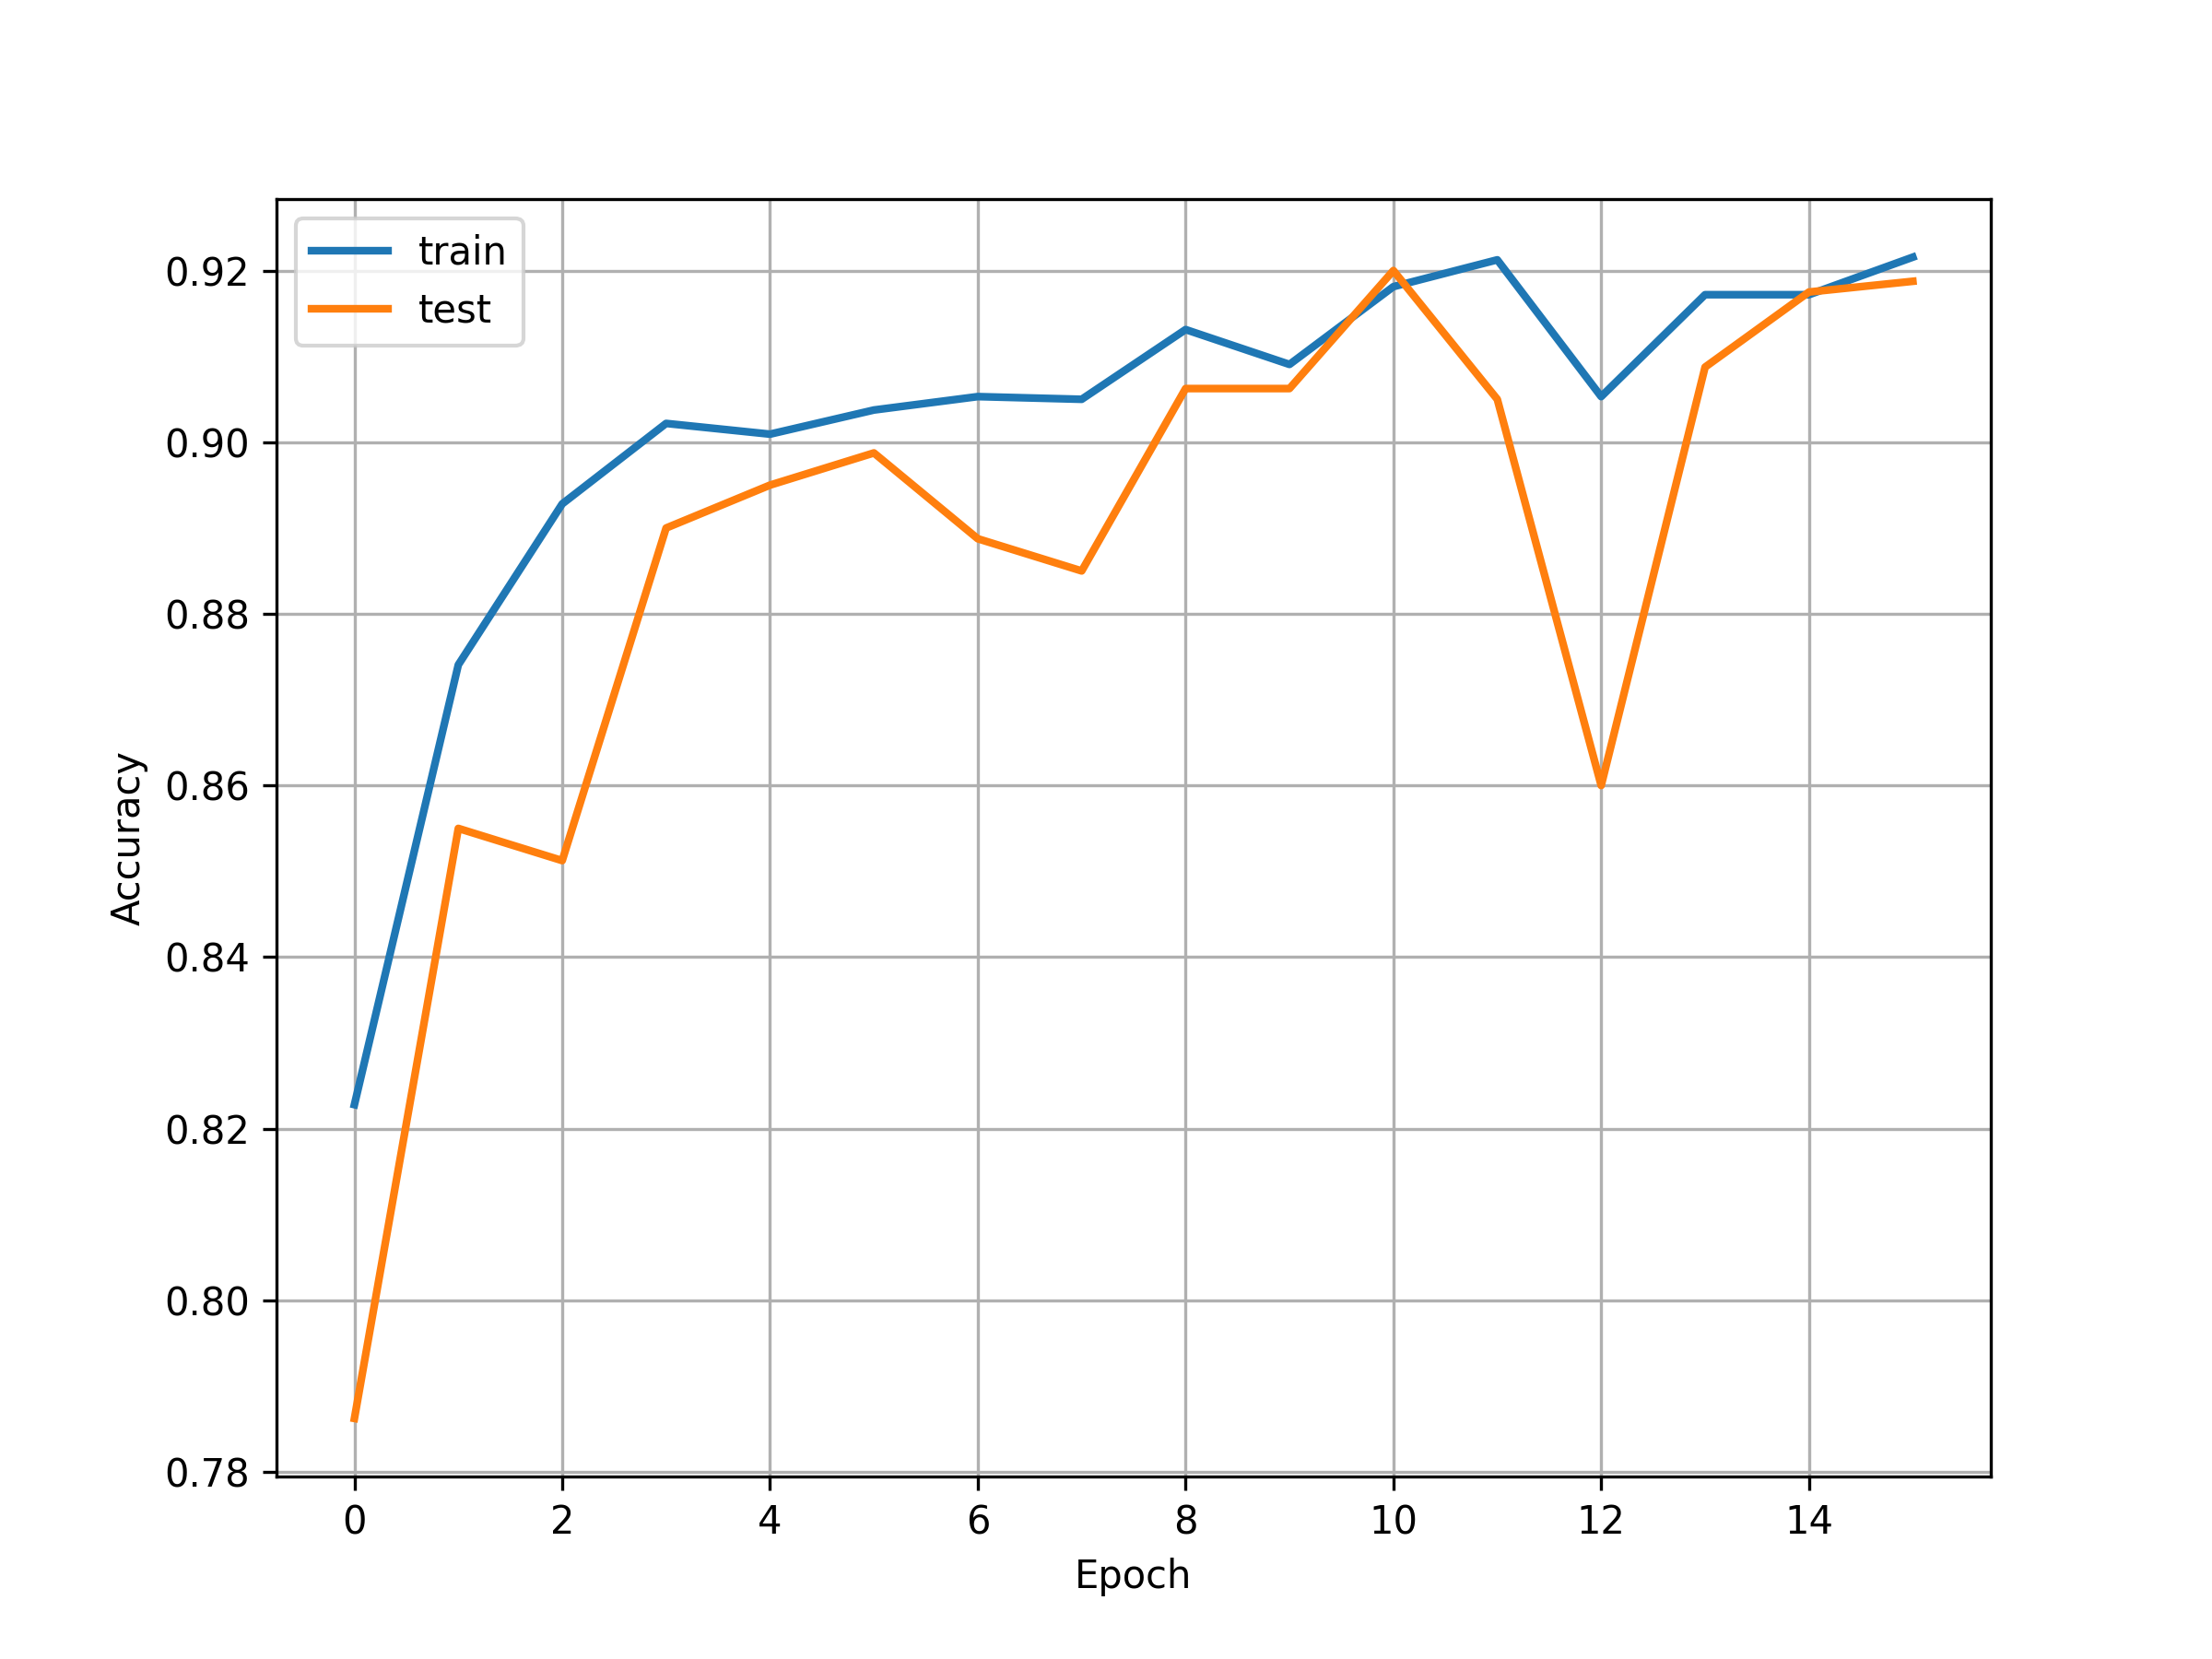
\includegraphics[width=\linewidth, trim=20 10 20 10, clip]{assets/accuracy_curve/resnet50_accuracy_curve.png}
			\caption{ResNet50 - Accuracy}
		\end{subfigure}
		\hfill
		\begin{subfigure}[b]{0.49\textwidth}
			\centering
			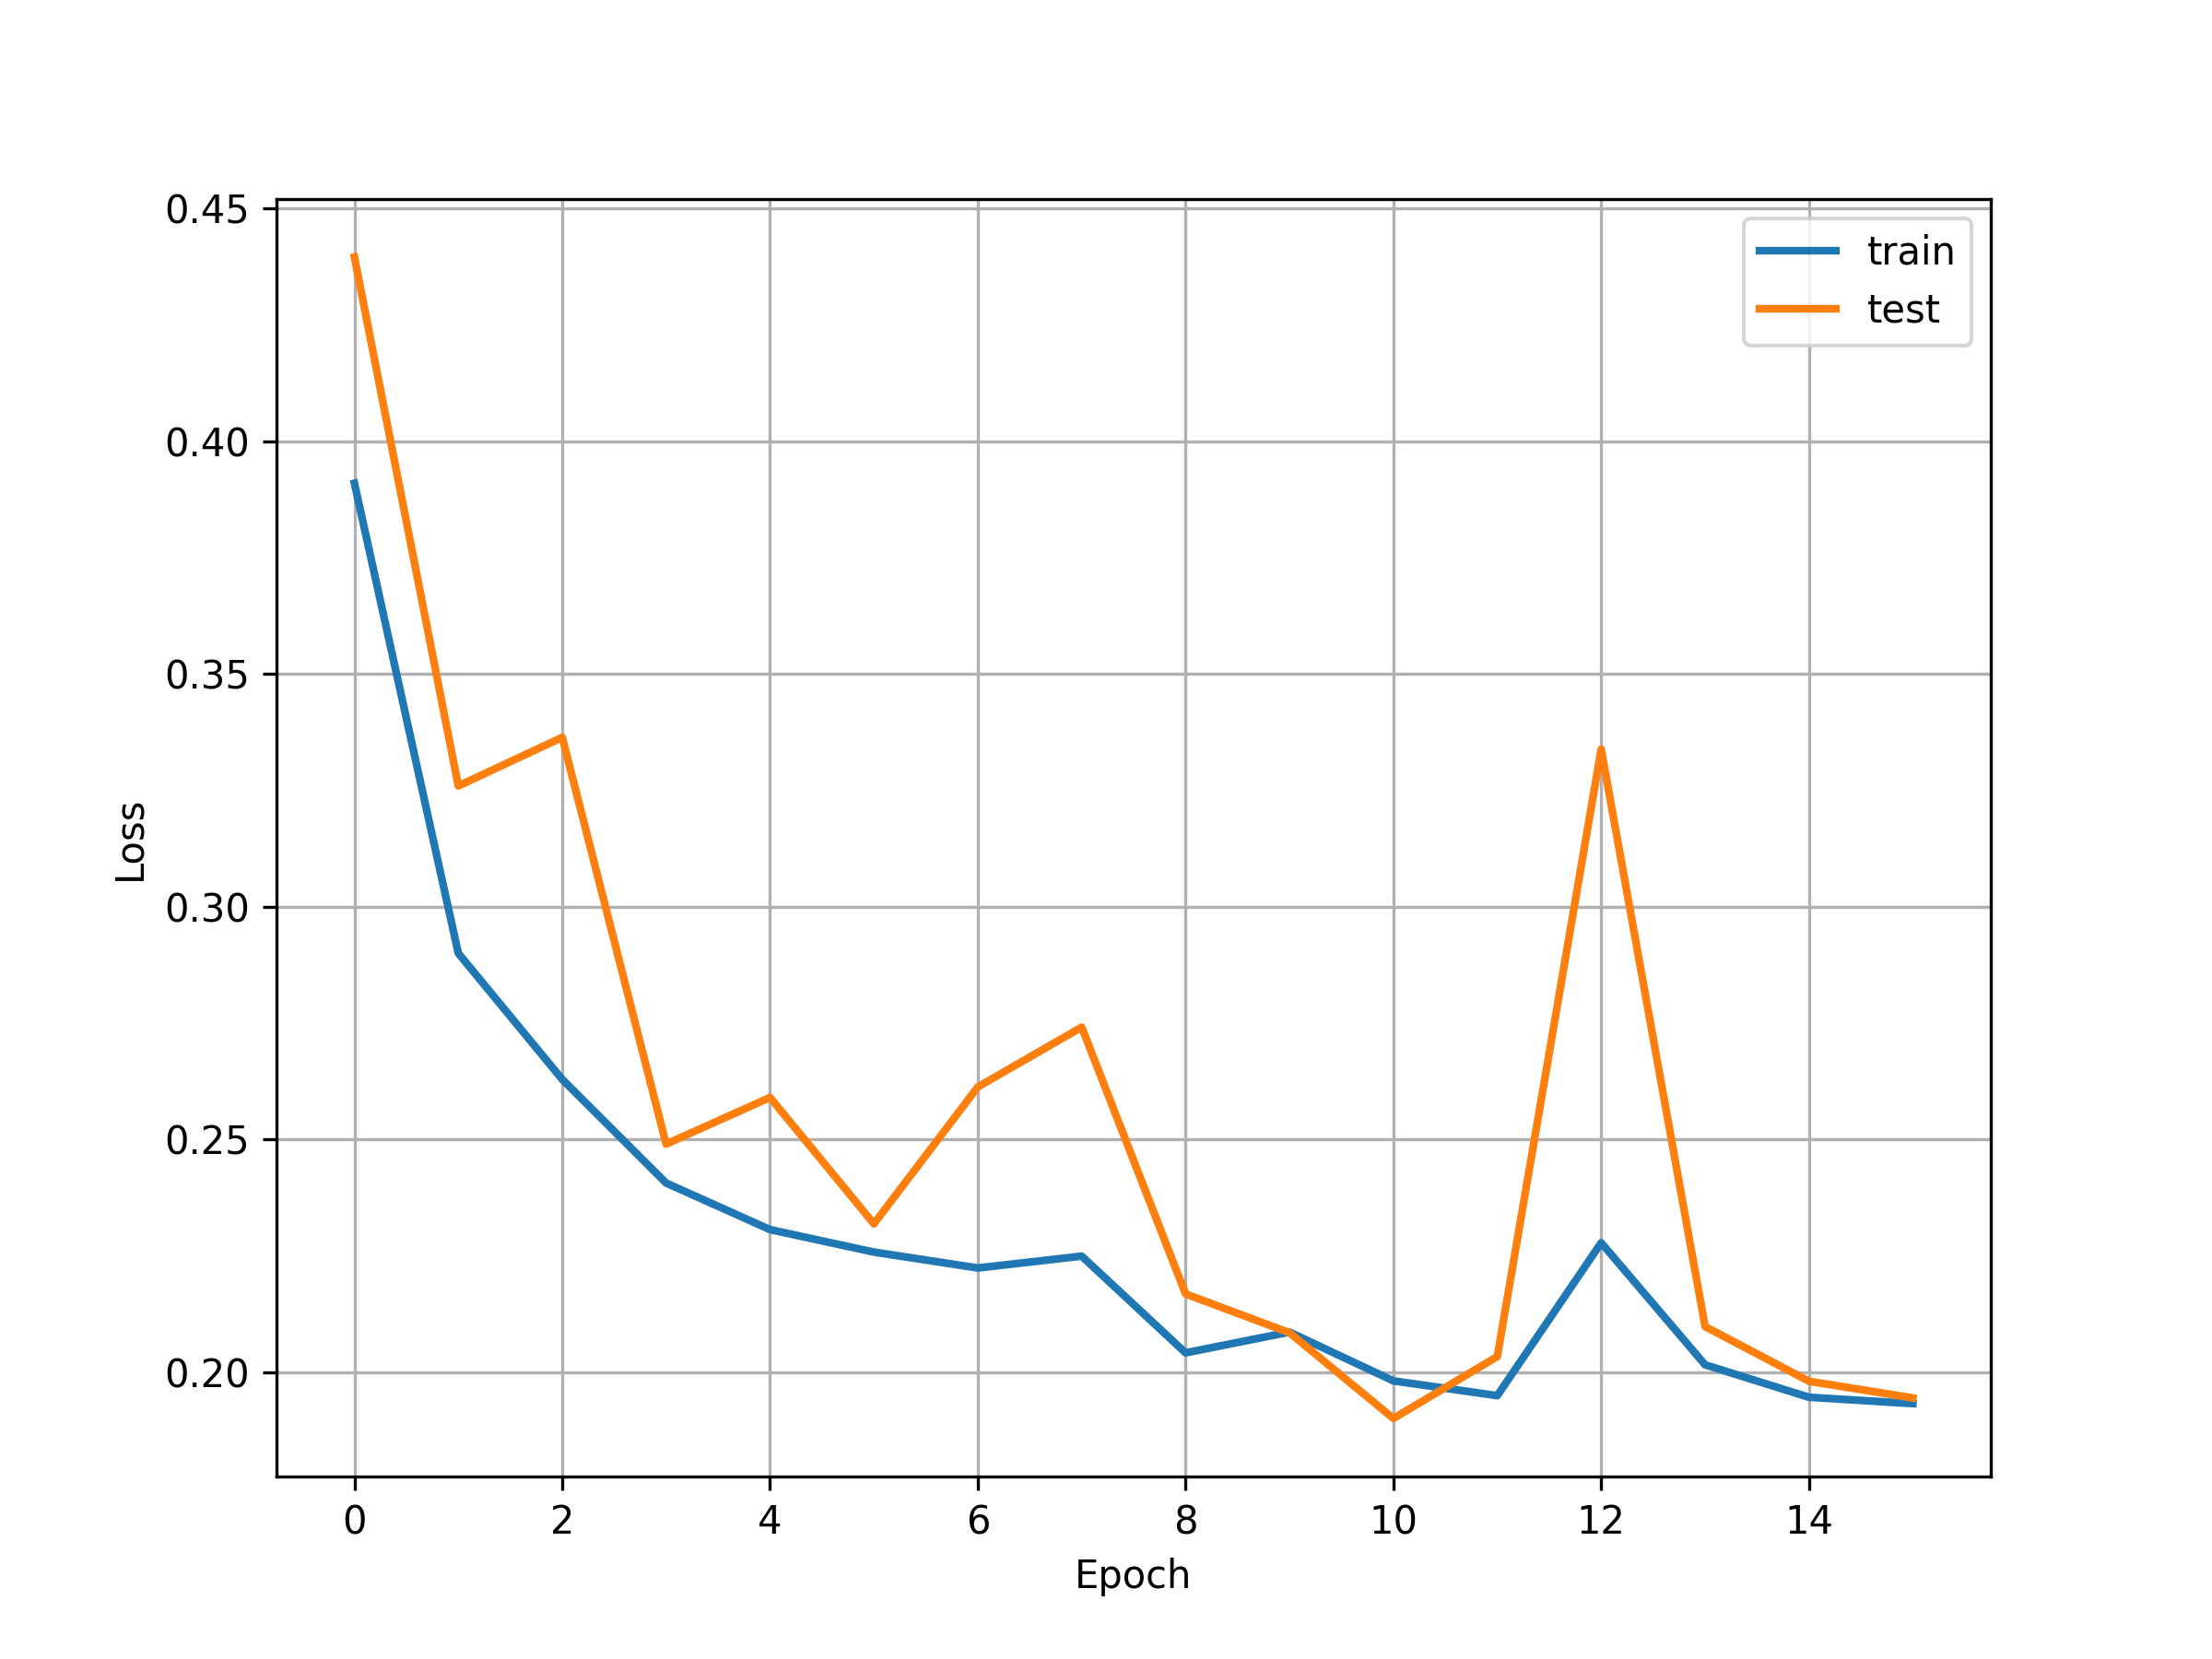
\includegraphics[width=\linewidth, trim=20 10 20 10, clip]{assets/loss_curve/resnet50_loss_curve.png}
			\caption{ResNet50 - Loss}
		\end{subfigure}
		
		% EfficientNet-B0
		\begin{subfigure}[b]{0.49\textwidth}
			\centering
			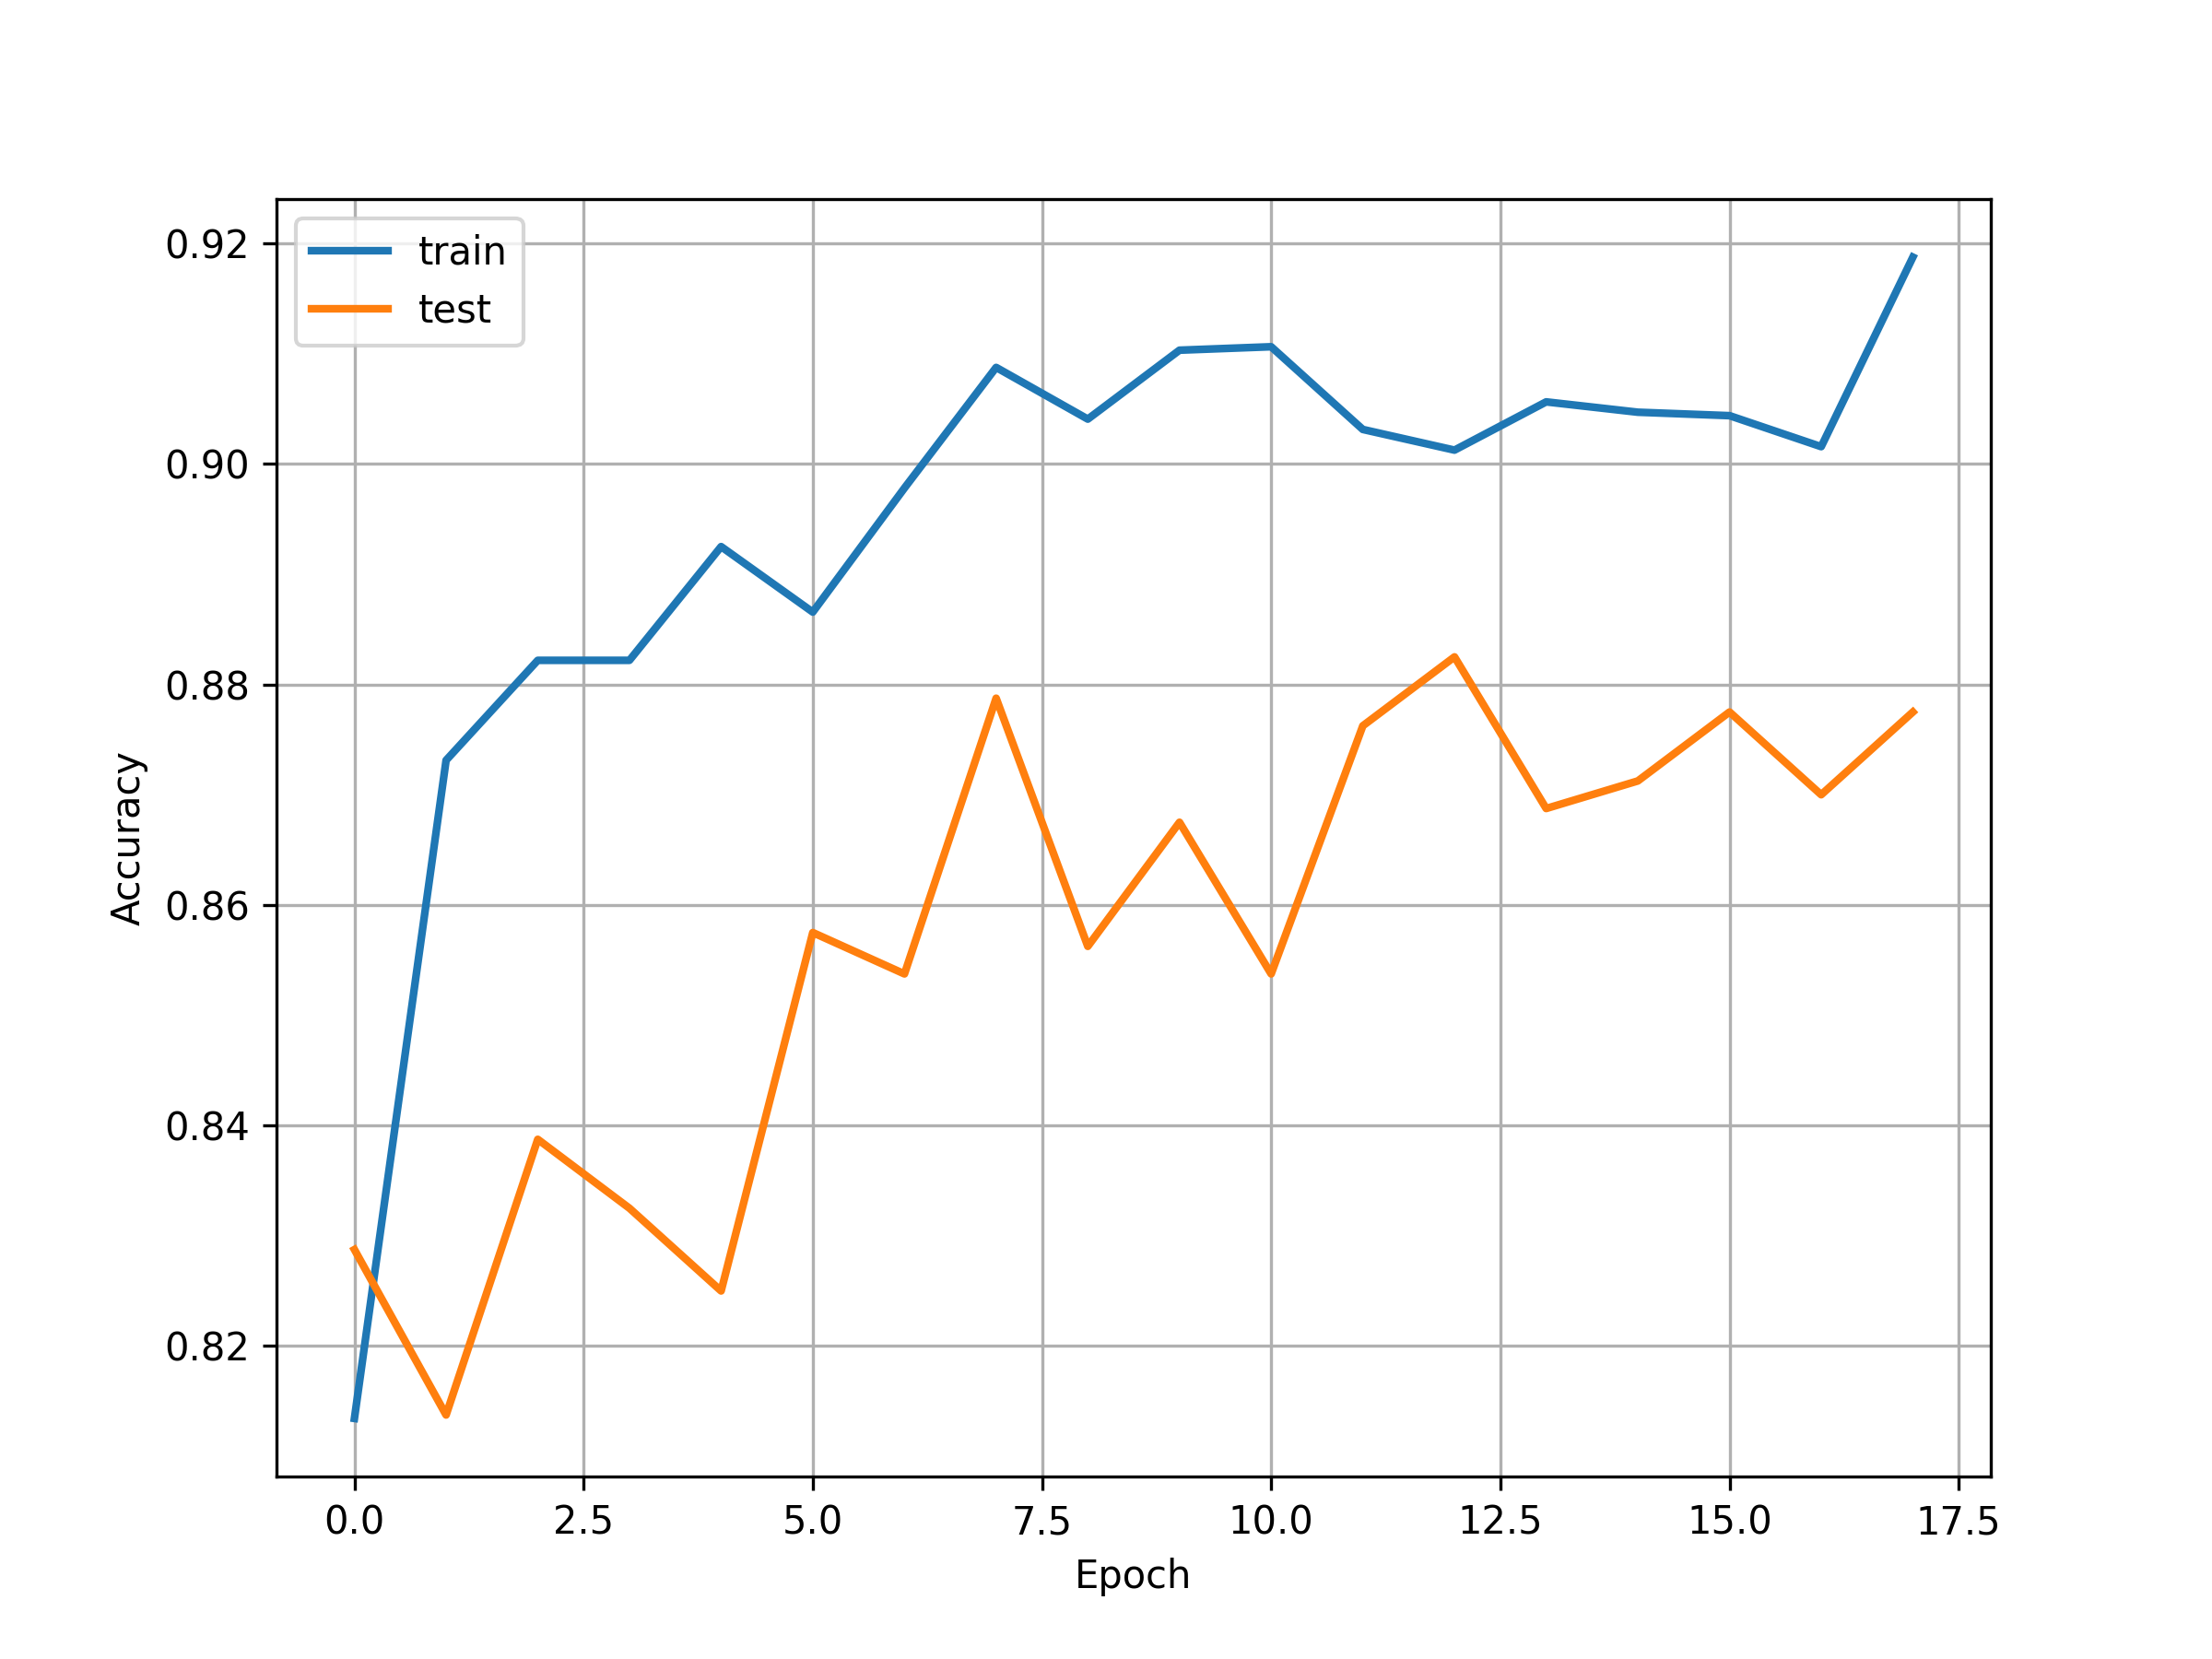
\includegraphics[width=\linewidth, trim=20 10 20 10, clip]{assets/accuracy_curve/efficientnet_b0_accuracy_curve.png}
			\caption{EfficientNet-B0 - Accuracy}
		\end{subfigure}
		\hfill
		\begin{subfigure}[b]{0.49\textwidth}
			\centering
			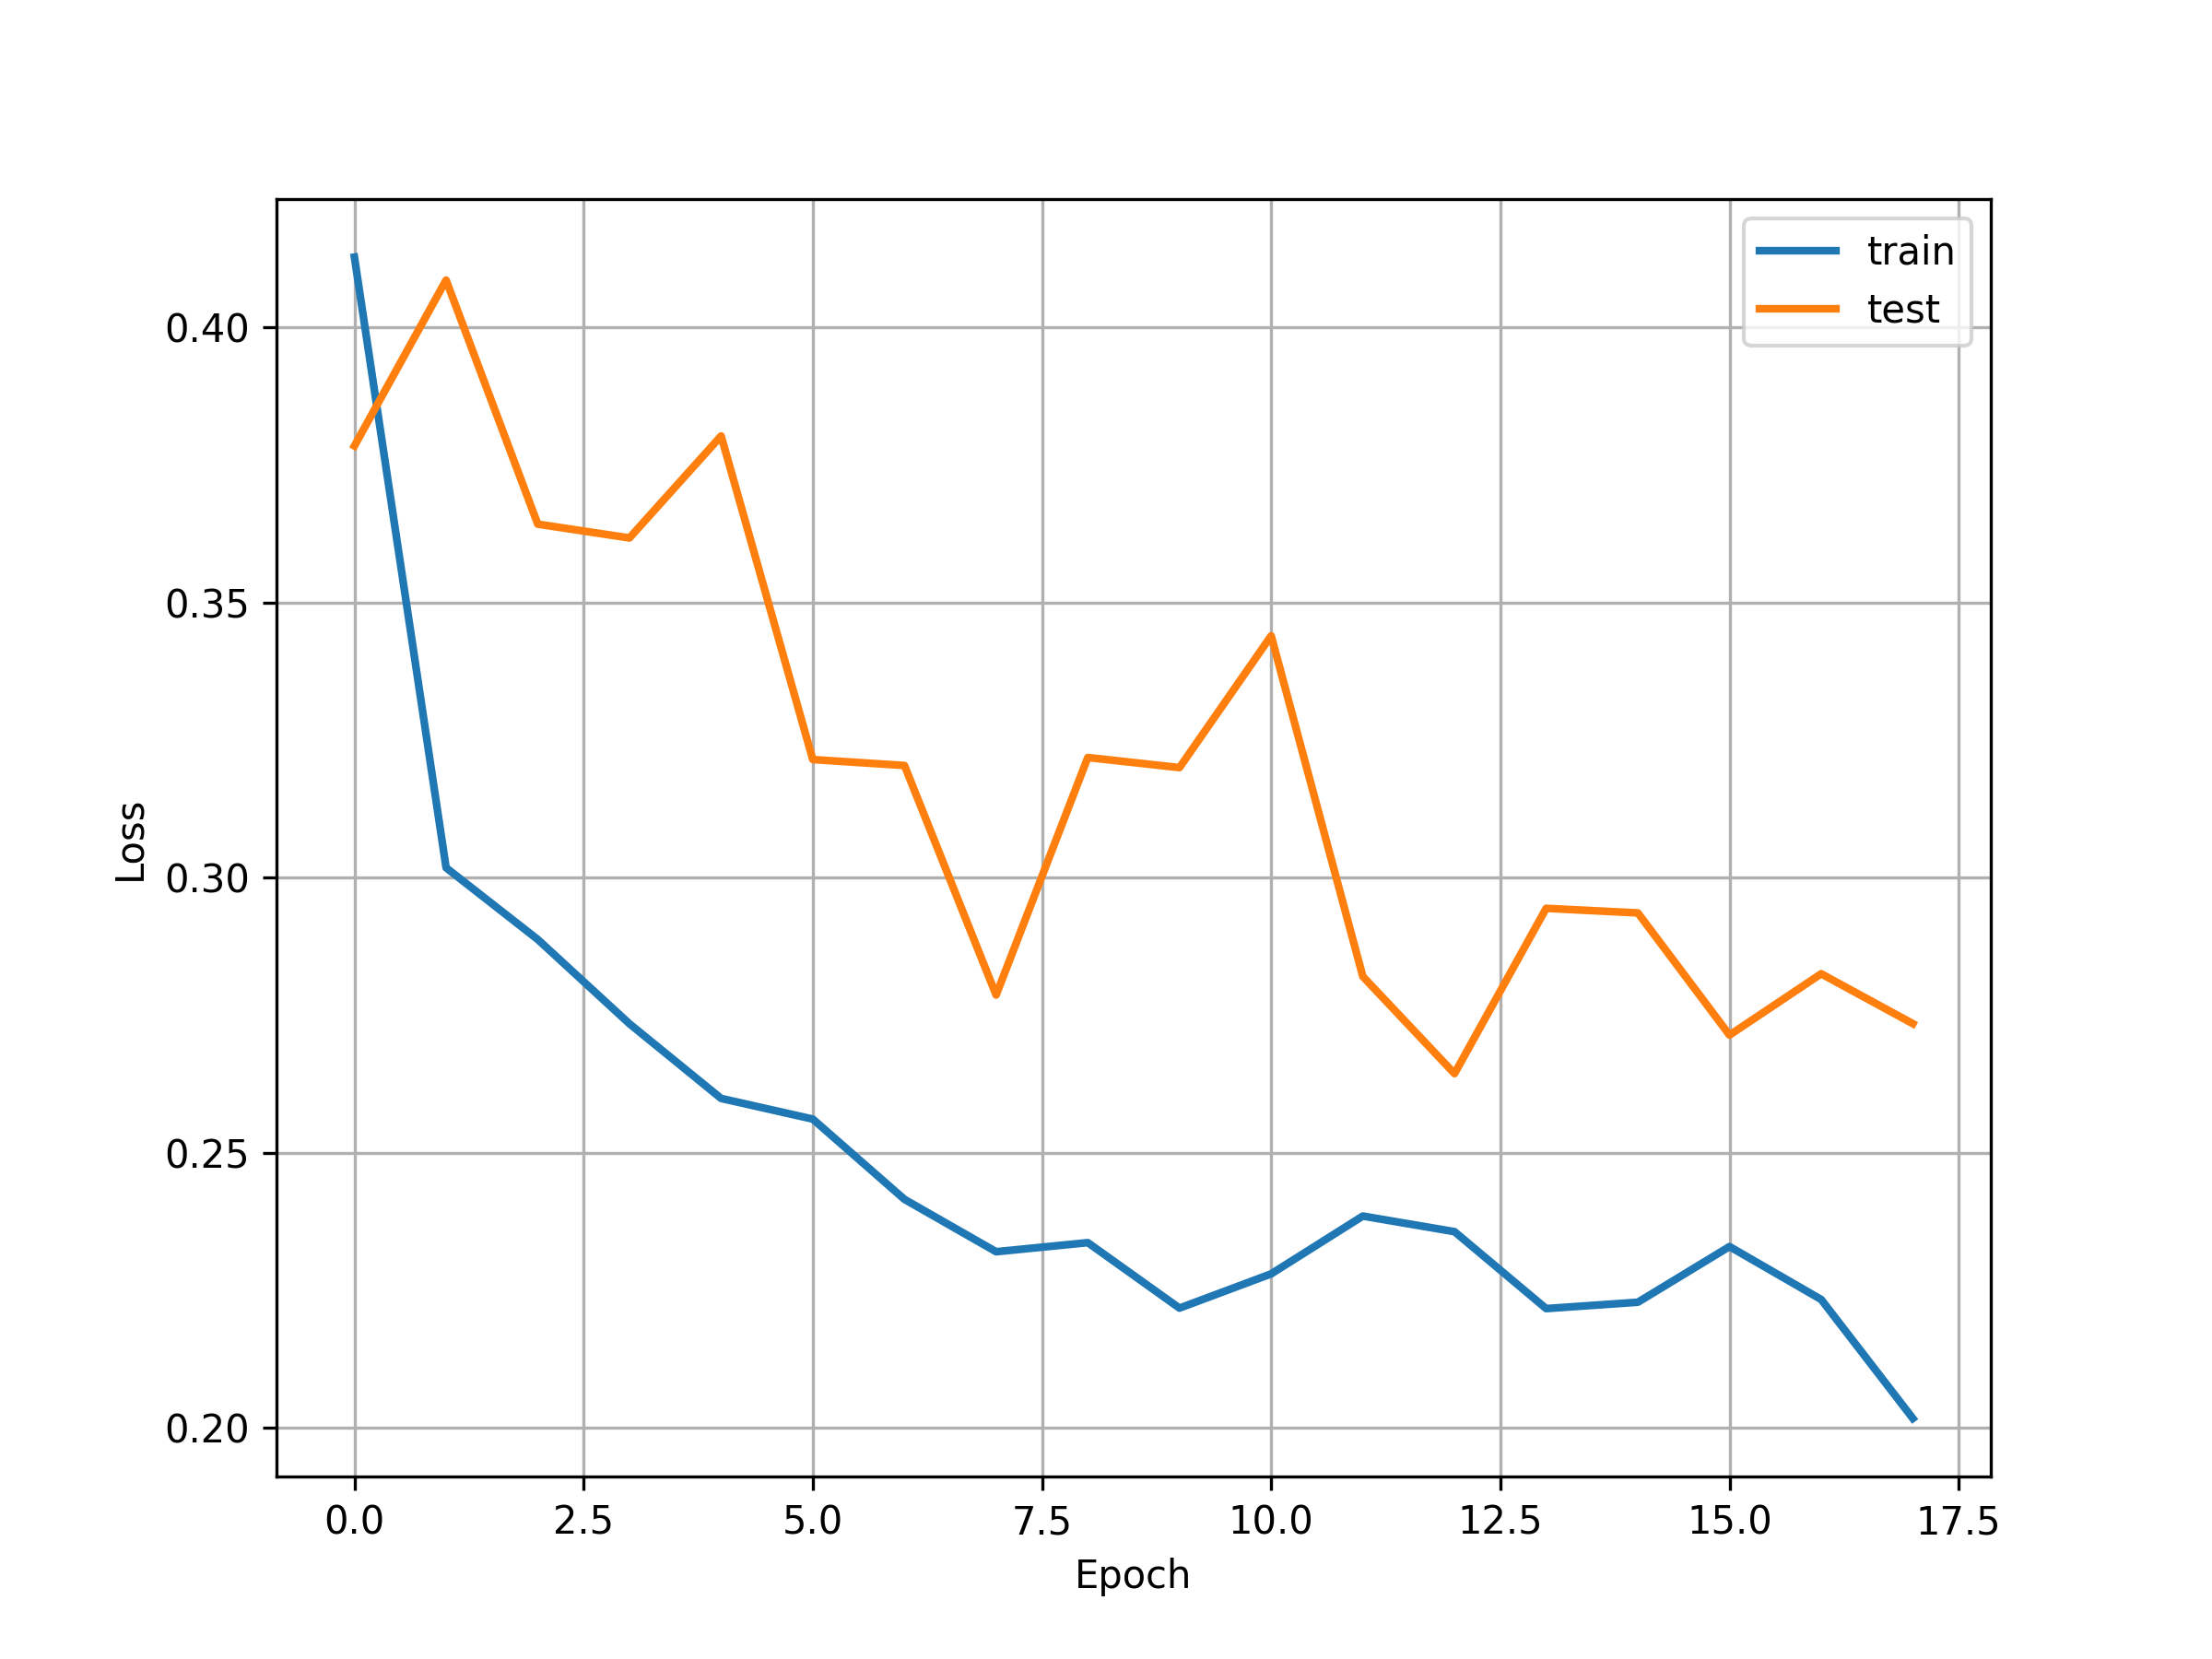
\includegraphics[width=\linewidth, trim=20 10 20 10, clip]{assets/loss_curve/efficientnet_b0_loss_curve.png}
			\caption{EfficientNet-B0 - Loss}
		\end{subfigure}
	\end{figure}
	
	Among the three models, VGG11 delivered the strongest overall performance, achieving the highest accuracy (95\%), precision (92\%), recall (94\%), and F1 score (93\%). Its confusion matrix shows 13 false negatives and 30 false positives—an acceptable outcome given the 3:1 class imbalance in the test set. This demonstrates VGG11's ability to minimise both missed detections and false alarms. The learning curves indicate stable training with minimal overfitting: test accuracy closely tracks—and occasionally exceeds—training accuracy, likely because the test set is less challenging than the randomly augmented training data. Test loss also declines steadily throughout training, with peak performance reached at epoch 24. These trends indicate strong generalisation and reliable convergence, positioning VGG11 as a robust candidate for operational maritime surveillance.
	
	ResNet50 also performed well, achieving 92\% accuracy, 88\% precision, 92\% recall, and a 90\% F1 score, with peak performance at epoch 11.  Although slightly less precise than VGG11, it maintained strong recall and generalisation. Its confusion matrix shows 16 false negatives and 49 false positives. A spike in test loss near epoch 12 suggests some volatility. ResNet50 may offer a favourable trade-off between accuracy and training efficiency when faster convergence is desirable.
	
	EfficientNet-B0, the most lightweight model, achieved 88\% accuracy, 83\% precision, and 90\% recall. While it matched VGG11 in terms of falses negatives (12), it producd the most false positives (86), indicating a tendency to over-predict hips. The learning curves show a clear gap between training and test loss, suggesting mild overfitting. Although it offers advantages in model size, the reduced precision may limit its usefulness in scenarios where false alarms are costly.
	
	\begin{figure}[H]
		\centering
		\caption{Sample Predictions and Ground Truth Labels}
		
		% VGG11
		\begin{subfigure}[c]{0.45\textwidth}
			\centering
			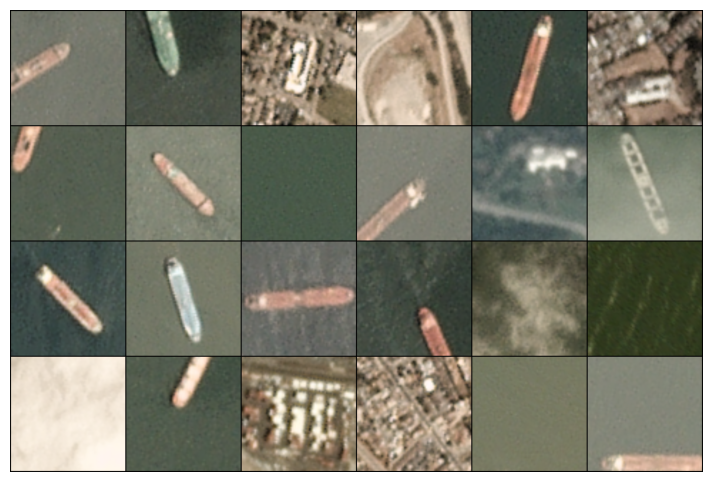
\includegraphics[width=\textwidth]{assets/sample_predictions/vgg11_sample_predictions.png}
		\end{subfigure}
		\hfill
		\begin{subfigure}[c]{0.45\textwidth}
			\centering
			\scriptsize
			\makebox[0.8\textwidth]{%
				\renewcommand{\arraystretch}{1.2}
				\begin{tabular}{l|cccccccccccc}
					\multicolumn{13}{c}{\textbf{VGG11}} \\
					\textbf{Predicted} & 0 & 0 & 0 & 0 & 1 & 0 & 0 & \cellcolor{red!20}0 & 0 & 0 & 0 & \cellcolor{red!20}0 \\
					\textbf{True}      & 0 & 0 & 0 & 0 & 1 & 0 & 0 & \cellcolor{red!20}1 & 0 & 0 & 0 & \cellcolor{red!20}1 \\
				\end{tabular}
			}
			
			\makebox[0.8\textwidth]{%
				\renewcommand{\arraystretch}{1.2}
				\begin{tabular}{l|cccccccccccc}
					\textbf{Predicted} & 1 & 1 & 1 & 0 & 0 & 0 & 0 & 0 & 0 & 0 & 0 & 0 \\
					\textbf{True}      & 1 & 1 & 1 & 0 & 0 & 0 & 0 & 0 & 0 & 0 & 0 & 0 \\
				\end{tabular}
			}
		\end{subfigure}
		
		% ResNet50
		\begin{subfigure}[c]{0.45\textwidth}
			\centering
			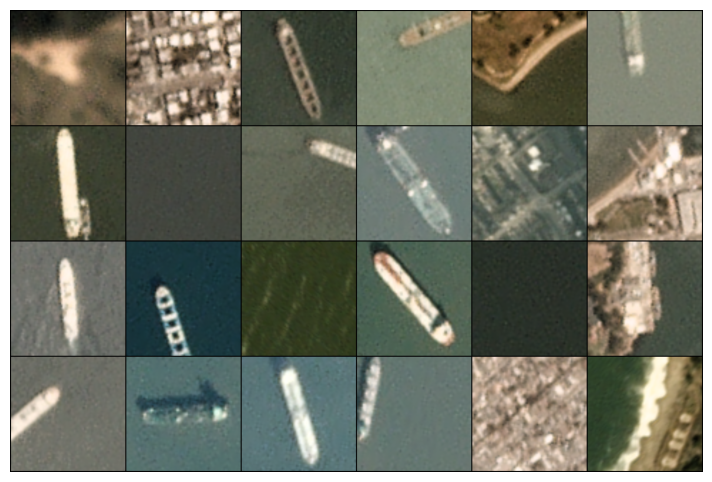
\includegraphics[width=\textwidth]{assets/sample_predictions/resnet50_sample_predictions.png}
		\end{subfigure}
		\hfill
		\begin{subfigure}[c]{0.45\textwidth}
			\centering
			\scriptsize
			\makebox[0.8\textwidth]{%
				\renewcommand{\arraystretch}{1.2}
				\begin{tabular}{l|cccccccccccc}
					\multicolumn{13}{c}{\textbf{ResNet50}} \\
					\textbf{Predicted} & 0 & 0 & 1 & 0 & 0 & 0 & 1 & 0 & 0 & 1 & 0 & 0 \\
					\textbf{True}      & 0 & 0 & 1 & 0 & 0 & 0 & 1 & 0 & 0 & 1 & 0 & 0 \\
				\end{tabular}
			}
			
			\makebox[0.8\textwidth]{%
				\renewcommand{\arraystretch}{1.2}
				\begin{tabular}{l|cccccccccccc}
					\textbf{Predicted} & 1 & \cellcolor{red!20}1 & 0 & 1 & 0 & 0 & 0 & \cellcolor{red!20}0 & 1 & 0 & 0 & 0 \\
					\textbf{True}      & 1 & \cellcolor{red!20}0 & 0 & 1 & 0 & 0 & 0 & \cellcolor{red!20}1 & 1 & 0 & 0 & 0 \\
				\end{tabular}
			}
		\end{subfigure}
		
		% EfficientNet-B0
		\begin{subfigure}[c]{0.45\textwidth}
			\centering
			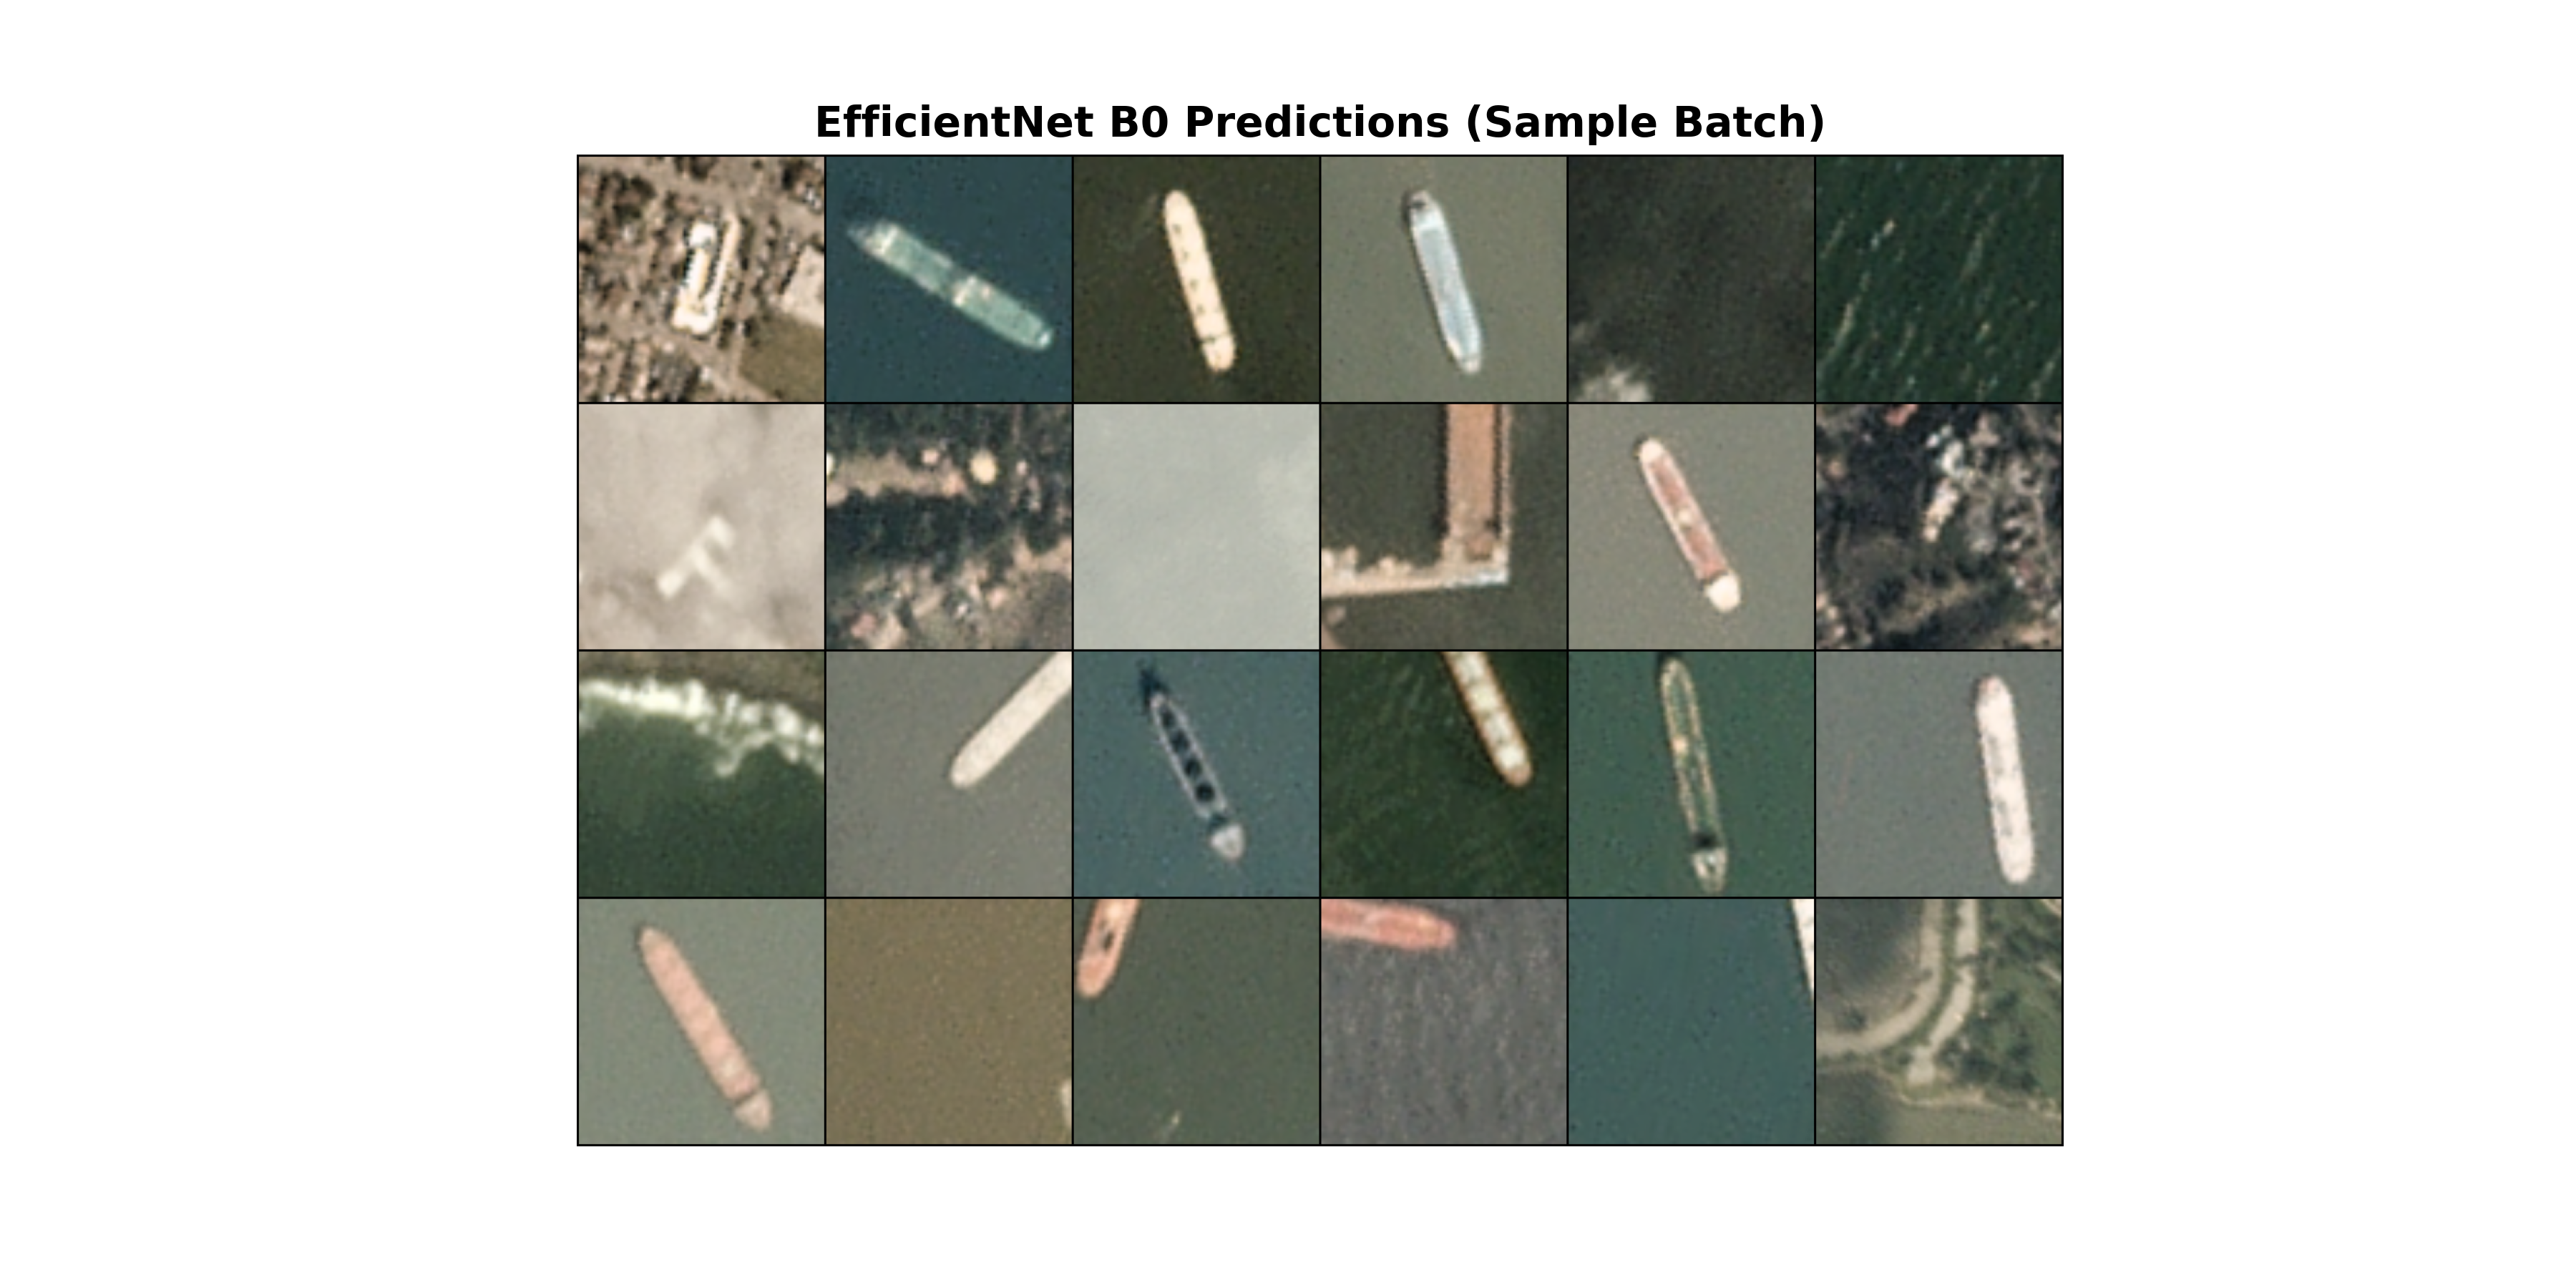
\includegraphics[width=\textwidth]{assets/sample_predictions/effnet_b0_sample_predictions.png}
		\end{subfigure}
		\hfill
		\begin{subfigure}[c]{0.45\textwidth}
			\centering
			\scriptsize
			\makebox[0.8\textwidth]{%
				\renewcommand{\arraystretch}{1.2}
				\begin{tabular}{l|cccccccccccc}
					\multicolumn{13}{c}{\textbf{EfficientNet-B0}} \\
					\textbf{Predicted} & 0 & 1 & 0 & 0 & 0 & 1 & 0 & 0 & 0 & \cellcolor{red!20}1 & 0 & \cellcolor{red!20}1 \\
					\textbf{True}      & 0 & 1 & 0 & 0 & 0 & 1 & 0 & 0 & 0 & \cellcolor{red!20}0 & 0 & \cellcolor{red!20}0 \\
				\end{tabular}
			}
			
			\makebox[0.8\textwidth]{%
				\renewcommand{\arraystretch}{1.2}
				\begin{tabular}{l|cccccccccccc}
					\textbf{Predicted} & 0 & 1 & 0 & 0 & 0 & 0 & 1 & 0 & 0 & \cellcolor{red!20}1 & 1 & 1 \\
					\textbf{True}      & 0 & 1 & 0 & 0 & 0 & 0 & 1 & 0 & 0 & \cellcolor{red!20}0 & 1 & 1 \\
				\end{tabular}
			}
		\end{subfigure}
	\end{figure}
	
	
	\vspace{-1em}
	
	\begin{figure}[H]
		\centering
		\caption{Occlusion-Based Attribution Maps}
		
		% First row: VGG11 and ResNet50 side by side
		\begin{subfigure}[b]{0.45\textwidth}
			\centering
			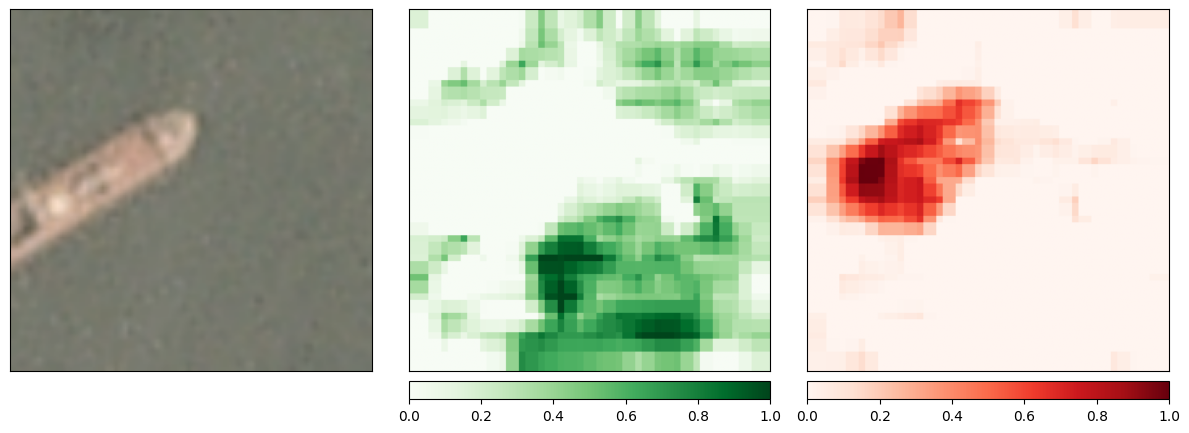
\includegraphics[width=\linewidth]{assets/occlusion/vgg11_occlusion.png}
			\caption{VGG11}
		\end{subfigure}
		\hfill
		\begin{subfigure}[b]{0.45\textwidth}
			\centering
			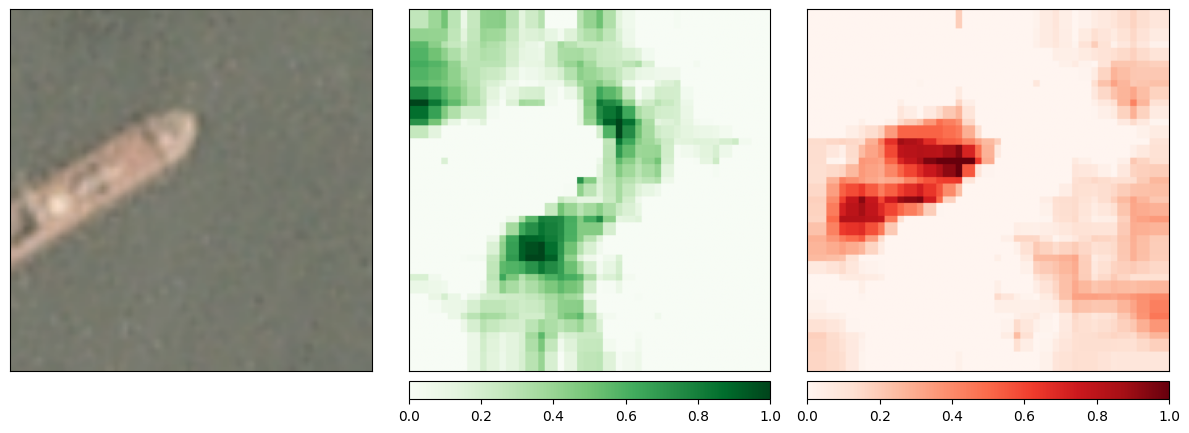
\includegraphics[width=\linewidth]{assets/occlusion/resnet50_occlusion.png}
			\caption{ResNet50}
		\end{subfigure}

		
		% Second row: EfficientNet-B0 centered
		\begin{subfigure}[b]{0.45\textwidth}
			\centering
			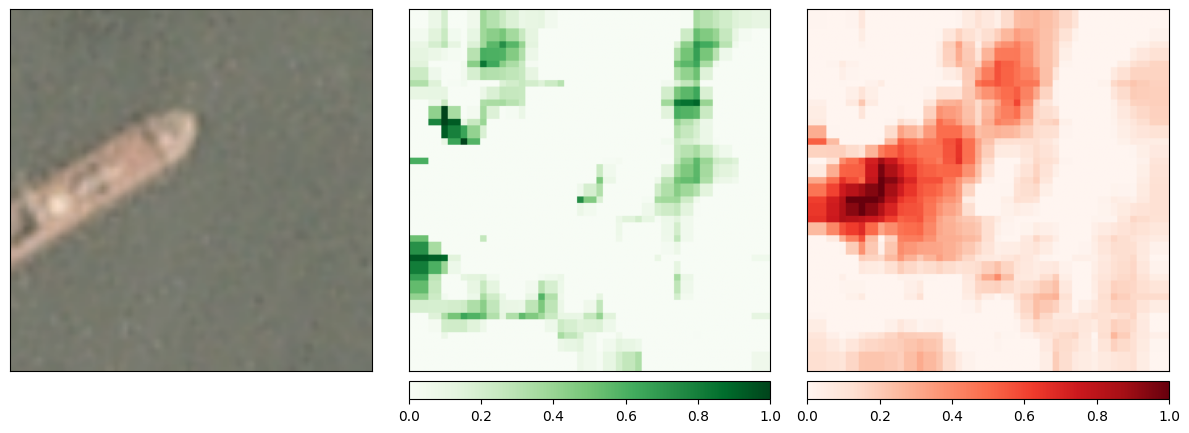
\includegraphics[width=\linewidth]{assets/occlusion/efficientnet_b0_occlusion.png}
			\caption{EfficientNet-B0}
		\end{subfigure}
	\end{figure}
	
	\begin{figure}[H]
		\centering
		\caption{Full-Scene Ship Detections and Confidence Heatmaps}
		
		% VGG11
		\begin{subfigure}[b]{0.49\textwidth}
			\centering
			\includegraphics[width=\textwidth]{assets/full_scene_detection/vgg11_detection_lb_2.png}
			\caption{VGG11 – Detection}
		\end{subfigure}
		\hfill
		\begin{subfigure}[b]{0.49\textwidth}
			\centering
			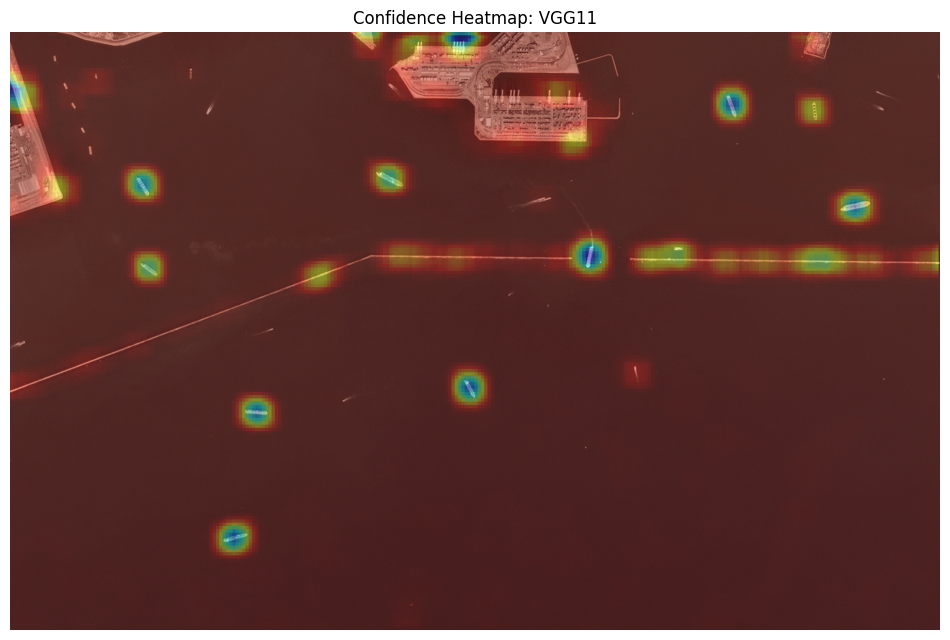
\includegraphics[width=\textwidth]{assets/confidence_heatmap/vgg11_confidence_heatmap.png}
			\caption{VGG11 – Heatmap}
		\end{subfigure}
		
		% ResNet50
		\begin{subfigure}[b]{0.49\textwidth}
			\centering
			\includegraphics[width=\textwidth]{assets/full_scene_detection/resnet50_detection_lb_2.png}
			\caption{ResNet50 – Detection}
		\end{subfigure}
		\hfill
		\begin{subfigure}[b]{0.49\textwidth}
			\centering
			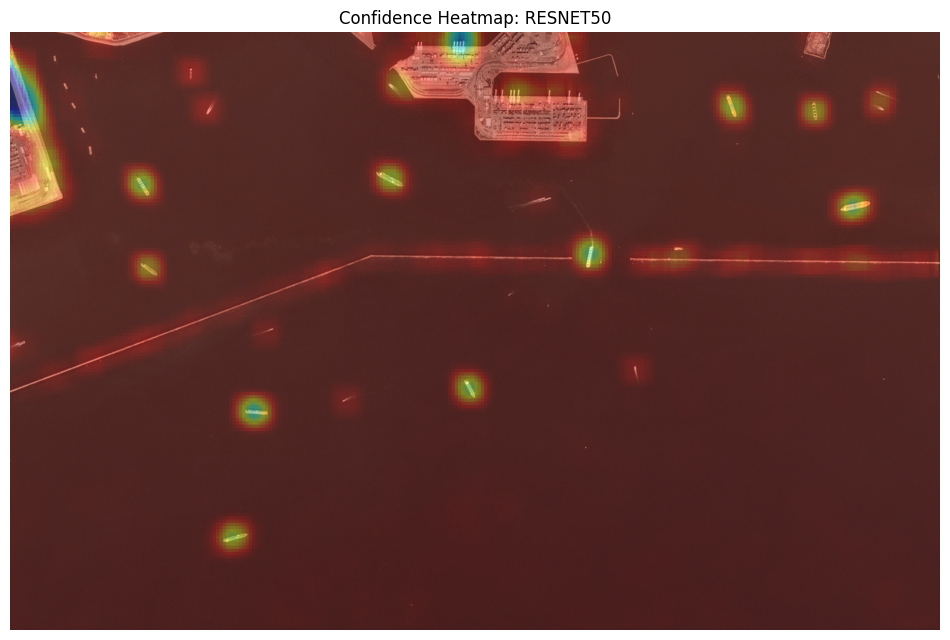
\includegraphics[width=\textwidth]{assets/confidence_heatmap/resnet50_confidence_heatmap.png}
			\caption{ResNet50 – Heatmap}
		\end{subfigure}
		
		% EfficientNet-B0
		\begin{subfigure}[b]{0.49\textwidth}
			\centering
			\includegraphics[width=\textwidth]{assets/full_scene_detection/efficientnetb0_detection_lb_2.png}
			\caption{EfficientNet-B0 – Detection}
		\end{subfigure}
		\hfill
		\begin{subfigure}[b]{0.49\textwidth}
			\centering
			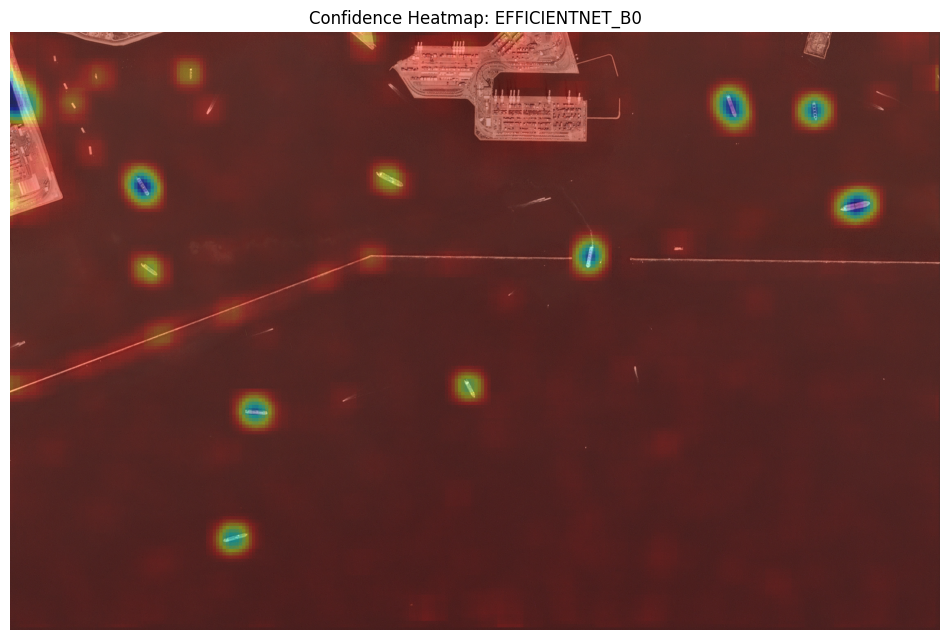
\includegraphics[width=\textwidth]{assets/confidence_heatmap/efficientnet_b0_confidence_heatmap.png}
			\caption{EfficientNet-B0 – Heatmap}
		\end{subfigure}

	\end{figure}
	
	To better understand model behaviour, we visualised predictions internal attention across different spatial scales. Figure 6 presents batch classification samples from each model. 
	
	\section*{Conclusion and Limitations}
	
	Observation of false positives. We observed some false alarms, mostly on features that resembled ships in size or colour. For instance, one image had a section of a pier that the model falsely highlighted (this is an example). This is likely due to the model's bias from the training set: many no-ship training chips contained ship-like elements, which can confuse the classifier.
	False positives could potentially be reduced by incorporating a water mask (so the model only scans areas known to be water)
	
	Window size constraint: using a fixed 80*80 window means the detector is tuned to ships of roughly that scale. If the ships in the scene is significantly larger than 80 pixels (e.g. a very large vessel) or much smaller, detection might be suboptimal. Our model requires the ship to mostly fit in the window to be confident. If the port image had ships larger than the chip size, the sliding window approach would still find them via multiple overlapping chips, but the model might see parts of a ship as "no-ship" if the ship is cut off. Advanced object detector would handle this via multi-scale feature maps
	
	Computation - sliding a window across an entire image is computationally expensive, though we mitigated it by batching predictions. A 3000 * 3000 pixel image would entail on the order of 9 million windows if done at every pixel - mention that using the GPU made this brute-force scanning feasible, but it won't scale well to very large or real-time use. Could further explore the use of YOLO.
	
	Environmental factors - note that our satellite images are optical (RGB) and presumably taken in clear conditions. The model would be challenged by clouds, extreme lighting changes, or if ships are camouflaged against backgrounds. Since it's trained on one specific port, it might not generalise perfectly to other ports without adaptation
	
	\newpage
	\begin{flushleft}
		\begin{thebibliography}{9}
			\bibitem{patel2022}
			Patel, K., Shah, J., Shah, M., and Shah, D.
			\textit{Deep Learning-Based Automatic Detection of Ships: An Experimental Study Using Satellite Images}.
			Journal of Imaging, 8(7), 2022.
			\url{https://doi.org/10.3390/jimaging8070182}
			
			\bibitem{rhammell2017}
			rhammell.\\
			\textit{GitHub - Rhammell/Shipsnet-Detector: Detect Container Ships in Planet Imagery Using Machine Learning}.\\
			GitHub, 2017.\\
			\url{https://github.com/rhammell/shipsnet-detector} (Accessed 27 Apr. 2025)
			
			\bibitem{zhao2024}
			Zhao, T., Wang, J., Li, Y., and Xie, H.\\
			\textit{Ship Detection with Deep Learning in Optical Remote-Sensing Images: A Survey of Challenges and Advances}.\\
			Remote Sensing, vol. 16, no. 7, 2024, pp. 1145--1145.\\
			\url{https://doi.org/10.3390/rs16071145} (Accessed 19 Aug. 2024)
			
			\bibitem{shipsnet2025}
			Rhammell.\\
			\textit{Ships in Satellite Imagery}.\\
			Kaggle, 2017.\\
			\url{https://www.kaggle.com/datasets/rhammell/ships-in-satellite-imagery/data} (Accessed 27 Apr. 2025)
			
			\bibitem{Kanjir2018} Kanjir, U.; Greidanus, H.; Oštir, K. (2018). *Vessel detection and classification from spaceborne optical images: A literature survey*. Remote Sensing of Environment, **207**, 1–26.
			
			\bibitem{Zhang2019} Zhang, S.; Wu, R.; Xu, K.; Wang, J.; Sun, W. (2019). *R-CNN-Based Ship Detection from High Resolution Remote Sensing Imagery*. Remote Sensing, **11**(6), 631.
			
			\bibitem{Bakirci2025} Bakırcı, M. (2025). *Advanced ship detection and ocean monitoring with satellite imagery and deep learning for marine science applications*. Regional Studies in Marine Science, **81**, 103975.
			
			\bibitem{Zhang2025} Zhang, B.; Liu, J.; Liu, R. W.; Huang, Y. (2025). *Deep-learning-empowered visual ship detection and tracking: Literature review and future direction*. Engineering Applications of Artificial Intelligence, **141**, 109754.
			
			\bibitem{Shi2025} Shi, W.; Zheng, W.; Xu, Z. (2025). *Ship-YOLO: A Deep Learning Approach for Ship Detection in Remote Sensing Images*. Journal of Marine Science and Engineering, **13**(4), 737.
			
			\bibitem{unctad2023}
			UNCTAD. \textit{Review of Maritime Transport 2023}. United Nations Conference on Trade and Development, 2023. \url{https://unctad.org/webflyer/review-maritime-transport-2023}
		\end{thebibliography}
	\end{flushleft}
\end{document}